\documentclass[conference]{IEEEtran}
\usepackage{xspace,shortcuts}
%\usepackage{times}
\usepackage{comment}
\usepackage{graphicx}
\usepackage{algorithm}
\usepackage{algorithmic}
%\usepackage{hyperref}
\usepackage{amsmath}
\usepackage{amssymb}
\usepackage{float}
%\usepackage{subfigure}
\usepackage{multirow}
\usepackage{courier}		% Used for coloring the table cells
\usepackage{url}
%\usepackage{bera}% optional: just to have a nice mono-spaced font
\usepackage{listings}
\usepackage{xcolor}
\usepackage{subcaption}
%\usepackage{floatrow}


\usepackage{booktabs} % For formal tables
\newcommand\qguan[1]{\textcolor{red}{(#1)}}
\newcommand\jchen[1]{\textcolor{blue}{(#1)}}
\newcommand\bluecomment[1]{\textcolor{blue}{// #1}}
\newcommand\redcomment[1]{\textcolor{red}{// #1}}
\newcommand\TOBEDONE[1]{\textcolor{red}{#1}}
% Copyright
%%\setcopyright{none}
%\setcopyright{acmcopyright}
%\setcopyright{acmlicensed}
%\setcopyright{rightsretained}
%\setcopyright{usgov}
%\setcopyright{usgovmixed}
%\setcopyright{cagov}
%\setcopyright{cagovmixed}
\usepackage{color,soul}
\usepackage{listings}


\lstset
{ %Formatting for code in appendix
    %basicstyle=\footnotesize
    numbers=left,
    %stepnumber=1,
    showstringspaces=false,
    tabsize=1,
    breaklines=true,
    breakatwhitespace=false,
    backgroundcolor=\color{backcolour}
}

\definecolor{backcolour}{rgb}{0.95,0.95,0.92}



\begin{document}
\title{Build and Execution Environment (BEE):
an Encapsulated Environment Enabling
HPC Applications Running Everywhere}



%\begin{comment}
\author{Jieyang Chen$^{*}$, Qiang Guan$^{\ddag}$, Xin Liang$^{*}$, Paul  Bryant$^{\ddag}$ Patricia Grubel$^{\dag}$, Allen McPherson$^{\dag}$,\\
  Li-Ta Lo$^{\dag}$,   
Timothy Randles$^{\dag}$, Zizhong Chen$^{*}$, and James Paul Ahrens$^{\dag}$ \\
$^{*}$University of California, Riverside 
$^{\ddagger}$ Kent State University 
$^{\dag}$Los Alamos National Laboratory \\
\{jchen098, xlian007, chen\}@cs.ucr.edu, 
\{qguan, pbryant1\}@kent.edu, \\
\{ pagrubel, mcpherson, ollie, trandles, ahrens\}@lanl.gov
}

%\end{comment}

\maketitle
%\thispagestyle{plain}
%\pagestyle{plain}

\linespread{0.97}%
\selectfont

\begin{abstract}
\begin{abstract}
Testing is one of the most important steps in software development. It ensures the quality of software. Continuous Integration (CI) is a widely used testing system that can report software quality to the developer in a timely manner during the development progress. Performance, especially scalability, is another key factor for High Performance Computing (HPC) applications. Though there are many applications and tools to profile the performance of HPC applications, none of them are integrated in the continuous integration. On the other hand, no current continuous integration tools provide easy-to-use scalability test capabilities.
%However, current CI only tests the software's functionality.  No current CI implementation provide . 
In this work, we propose BeeSwarm, a scalability test system that can be easily applied to the current CI test environment enabling scalability test capability for HPC developers. As a showcase, BeeSwarm is integrated into Travis CI and executes the scalability test workflow on Chameleon cloud. 
%\pat{Do you have a reference for Chameleon?}
%\qguan{This is qguan}

\end{abstract}
\end{abstract}

% add page number


%\footnotetext[1]{The
%publication has been assigned the LANL identifier LA-UR-17-26423.}


\begin{IEEEkeywords}
high performance computing; cloud computing; container.
\end{IEEEkeywords}
%\footnotetext[1]{The publication has been assigned the LANL identifier LA-UR-18-27912.}

%\linespread{1}%
%\selectfont
\section{Introduction}
High software quality is one of the most important goal of software development. Software testing serves as the most widely used approach to ensure the quality of softwares meet expectation.
%Software testing is one of the most important processes in HPC software development. 
A good way to test software is to include automated tests in the build process.  With the rise of Extreme Programming (XP) and Test Driven Development (TDD), self-testing processes for code development have become popular and are widely adopted by many software development projects. 
As softwares become increasingly structurally complicated, the number of developers involved in the development process increases. As each developer makes progress, they commit their work periodically (every several hours or days) to the central code repository (e.g., git, SVN). Not only does each developer's work require testing, the integration of work between developers also requires testing. So, Continuous Integration (CI) \cite{fowler2006continuous} is widely adopted in many software development projects. A CI server is used dedicatedly for testing. Each time a developer makes a commit of her work to the central code repository, the CI server automatically make a clone of the project and conduct pre-designed tests, so that it can constantly monitor the quality of the software in terms of correctness and report potential problems in a timely fashion, helping developers make bug fixes more efficiently.  %\pat{I wouldn't say the servers mimic the production env.}
%\pat{what is this a hanging here for}

\begin{figure*}[h]
    \centering
    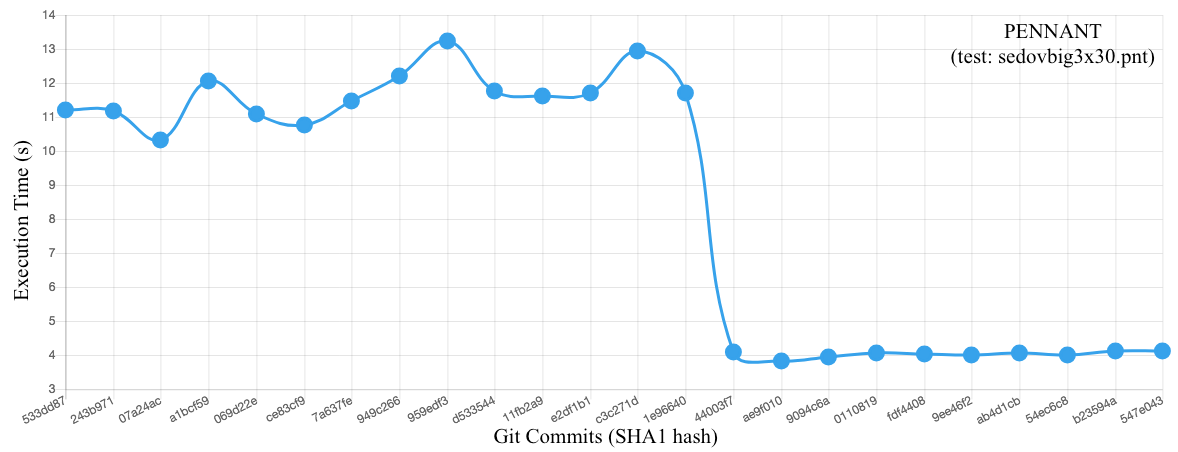
\includegraphics[width=1\textwidth]{figures/CI-motivation-2.png}
    \caption{Example: the performance of Legion \cite{bauer2012legion} changes as developers make progress. The performance is obtained by running a benchmark PENNANT\cite{ferenbaugh2015pennant} on the Legion system. The test suit sedovbig3x30 running on 10 processes (CPU cores) is used. 
%\textcolor{red}{Caption should be changed because this perforamnce is about Legion not PENNANT.}
}
    \label{exp}
\end{figure*}


When it comes to HPC applications, \textit{performance} and \textit{scalability} %large-scale
%\trandles{Remove 'large-scale' here because you have it at the end of the sentence} 
are the other two important factors of software quality besides correctness, since the application are usually designed to deliver high performance on given platforms. Also applications that aim to solve complex time-consuming problems are expected to obtain good speedup when deployed on multi-node clusters, many-core architectures, or large-scale supercomputers. The scalability of HPC application is usually interpreted as how much speed up can be obtained given more computing resources. Better scalability means that the HPC application can use the underlying computing resources more efficiency and constantly deliver good performance on a various amount of computing resources.

During the HPC application development, as developers make progress,
%\pat{not sure if I changed your meaning here}
and they commit their work to the central code repository, the scalability of the application can change. For instance, it can be caused by changes in algorithm design, tunable parameters, and different hardware architectures of target production systems. For example, \textbf{Fig. \ref{exp}} shows the  performance of Legion \cite{bauer2012legion}, a data-centric parallel programming system, changes %\pat{shouldn't you explain what Circuit is I assume it's some sort of simulation, is it really an HPC code or just a benchmark code? Also, the axes of figure need to be labels I have no idea what they are}
%\trandles{Change the data point styles on the graph and refer to them by the symbols instead of colors.  Color-blind readers won't be able to easily distinguish between the two data series as presented.}
with different source code commits. The performance is obtained by running a benchmark software, PENNANT\cite{ferenbaugh2015pennant}, on the Legion system. As we can see the execution time can significantly change as developers make progresses. Receiving performance or scalability results like this in a timely manner can greatly help developers make better decisions about their code design and deliver HPC software with expected quality. However, current designs of CI services are commonly focused on monitoring the software quality in terms of correctness (e.g., detecting software bugs). To the best of our knowledge, none of the current works can easily enable automatic performance or scalability tests in CI since the test environment of CI is usually deployed on a single machine incapable of conducting large-scale scalability test.

\begin{figure}[h]
    \centering
    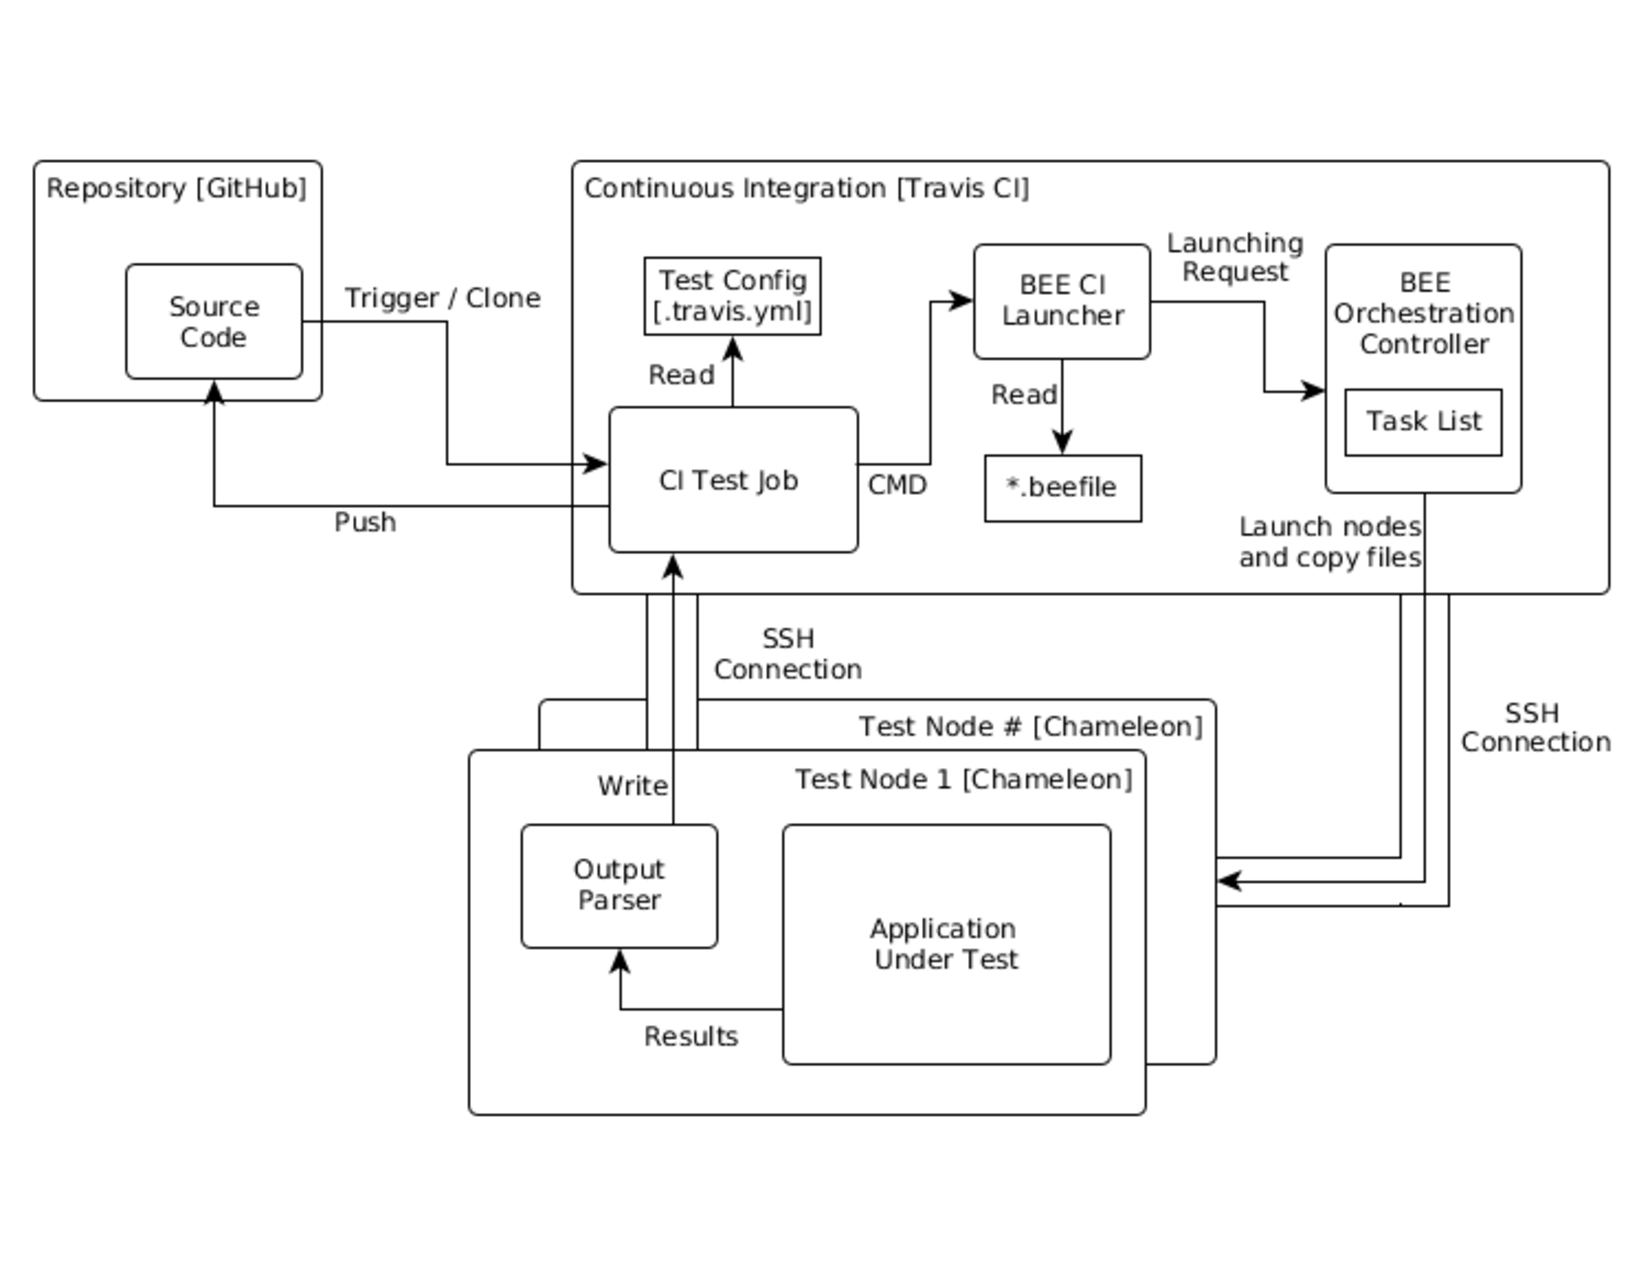
\includegraphics[width=0.5\textwidth]{figures/beeSwarm_Arch_ver02.pdf}
    \caption{Architecture of \texttt{BeeSwarm}. %\textcolor{red}{****Figure is not readable}
    }
    \label{arch}
\end{figure}


In this work, we propose a performance and scalability test system for CI -- \texttt{BeeSwarm}. \texttt{BeeSwarm} can be used as a plug-in for any current CI service. It takes the widely used Docker container as input, and the performance and scalability test can run on both HPC cluster environments and cloud computing environments. Just like the original correctness test in CI, the performance and scalability test are also autonomic. It only requires users to make simple specifications about the test environment they want to use and the test specification they need. Every time developers commit a change to the central code repository, they can choose to schedule a scalability test after the success of original correctness test. The performance and scalability test results will be automatically pushed back to the central code repository. %\pat{can this be controlled, maybe they don't want every change to spawn a scalability test}
Although we deploy \texttt{BeeSwarm} on Travis CI in this work, it can also be deployed on any other CI test environment. To deploy on another CI platform, only minimum modifications to the \texttt{BeeSwarm} configuration scripts are necessary, which makes \texttt{BeeSwarm} highly portable across CI platforms. In addition, although we only show the use of Chameleon cloud, the scalability test can also be executed on any other BEE-supported platform (HPC clusters, AWS, OpenStack, etc). This gives developers the flexibility to choose the platform they want their applications to run on.

The rest of this paper is organized as follows. We motivate our work in section \ref{motivation}. In section \ref{background}, we give necessary background that can help readers understand this work. We provide design details of \texttt{BeeSwarm} in section \ref{design} followed by experimental evaluation in section \ref{experiments}. Section \ref{related_work} discuss recent works that related to ours. Finally, section \ref{conclusion} concludes our work. %\textcolor{red}{Please change this accordingly after adding the motivation session}

\begin{figure*}[h]
    \centering
    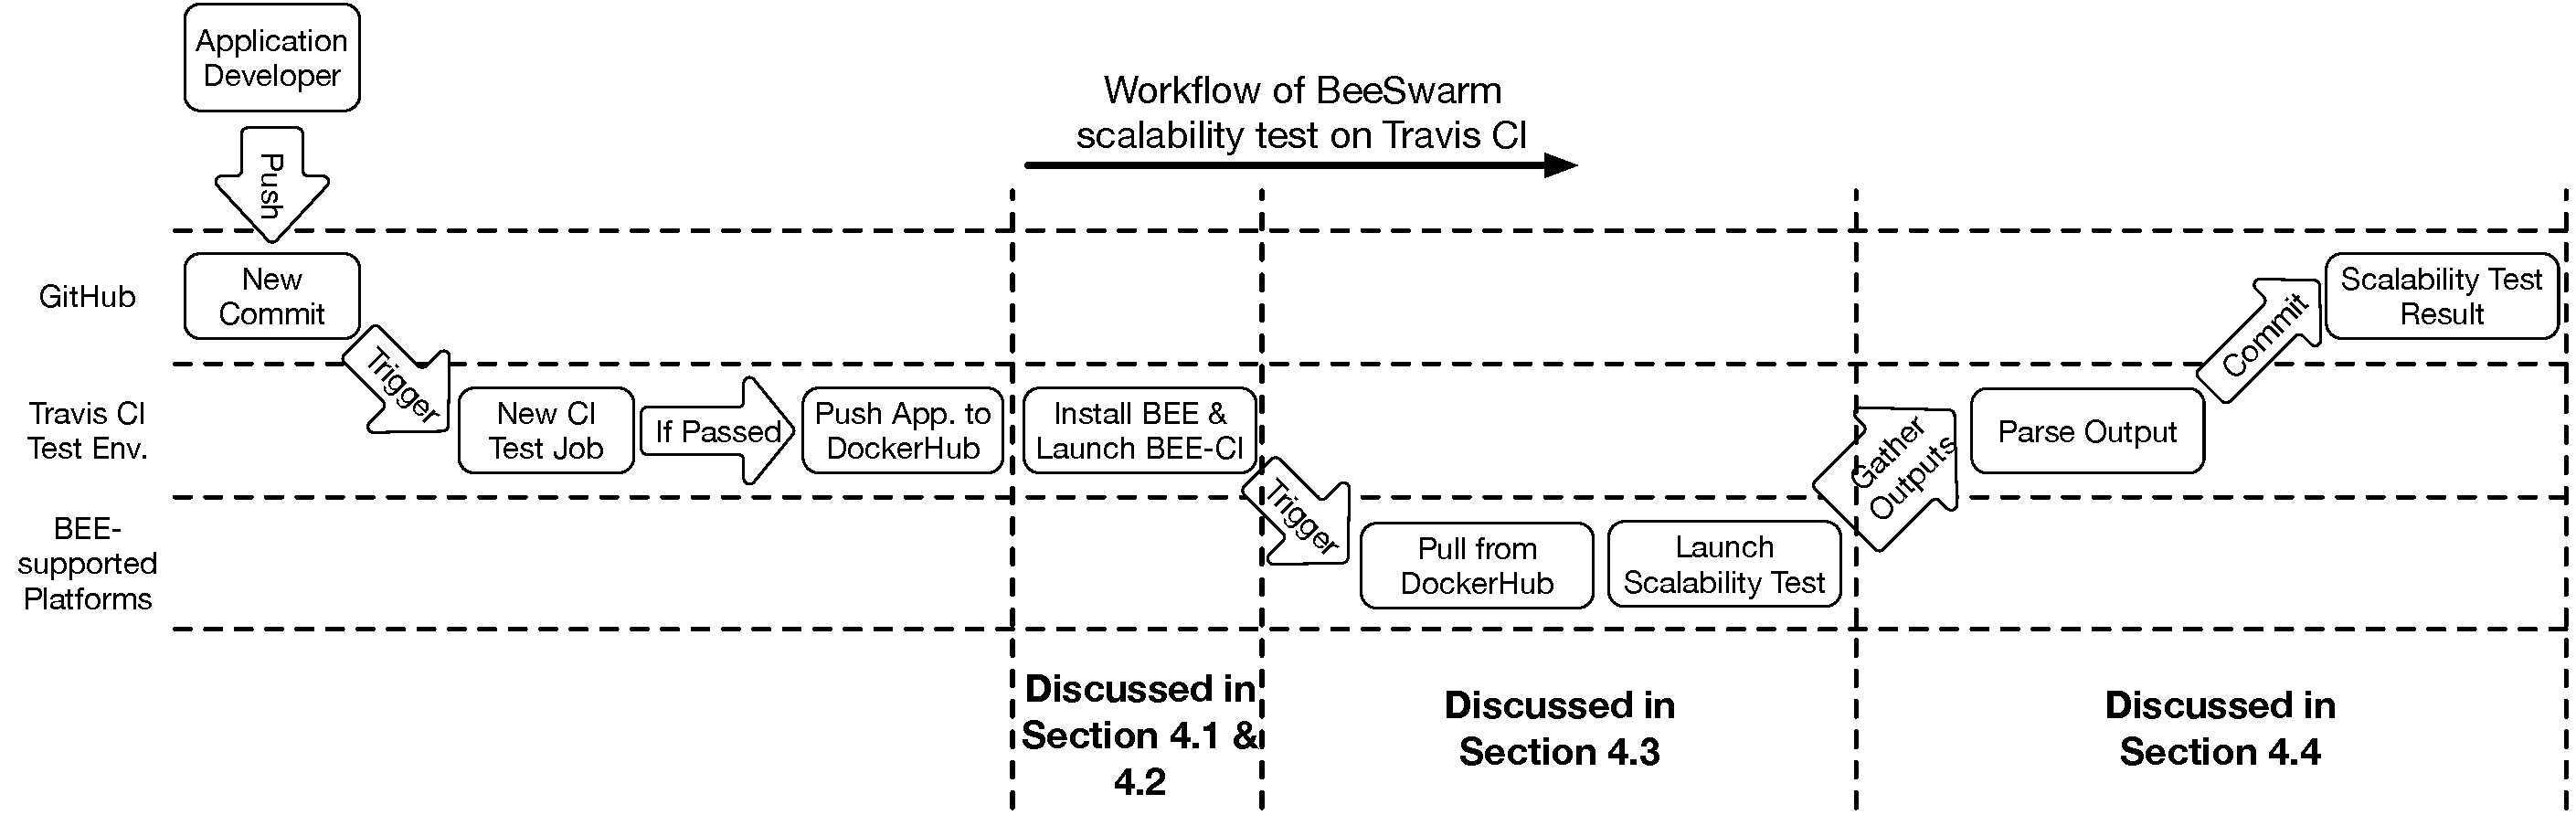
\includegraphics[width=1\textwidth]{figures/CI-workflow.pdf}
    \caption{Overall Workflow of BeeSwarm CI Scalability Test. 
    %\textcolor{red}{Can we add some horizontal lines to partition the steps of workflow to make them mapping 4.1-4.4? And move this graph to page 3, on top of it.}
    }
    \label{overall}
\end{figure*}


\section{BEE design overview}
\label{bee-framework-section}
The goal of \texttt{BEE} is to enable unified experience for users when launching HPC applications across different platforms. This is manifested in two ways: (1) A unified user interface that only requires minimum configuration to launch applications on a platform or switch between different platforms; (2) Similar execution environments for applications on different platforms that enable consistent application execution behavior.

\subsection{User interface}


The unified user interface consists of three inputs when launching an application using \texttt{BEE}:
\begin{enumerate}
\item A Docker image containing the application;
\item Run scripts;
\item Task description file -- \texttt{beefile};

\end{enumerate}
The first input is the Docker image containing the application. Then, to run the application when it is deployed on a platform, users need to provide run scripts. Depending on the application, the scripts can be in many forms e.g., Shell scripts, Python scripts, etc. Both the Docker image and run scripts do not need to be modified when switching between different execution platforms. Finally, to hide most complications and still provide enough capability of customization, we propose to use a simple JSON-format task description file (\texttt{beefile}) to handle all the communications between users and \texttt{BEE}. \textbf{Listing 1} shows the template of a \texttt{beefile}. Users need to select the suitable execution platform (line 3), provide general sequential run scripts (line 5 - 9) and MPI parallel run scripts (line 10 - 14), information about Dockerized  application (line 16 - 20), and finally provide necessary platform-specific information (line 21 - 26) e.g., node list, credential information. Note different Docker containers, by default, do not share a file system at runtime, but many HPC application processes running on different nodes need to have a shared directory to share data, so \texttt{BEE} needs users to specify a directory inside the container (line 16) that will be mounted to a shared host filesystem at runtime. When switching between platforms, users only need to make modifications to the \texttt{beefile}.

\lstset{numbers=left,
xleftmargin=1.5em,
frame=single,
framexleftmargin=2em}


\lstset{language=Java}
\begin{lstlisting}[ float, escapechar=!,
				   caption= Template of \texttt{beefile}]
 "task_conf": {
  "task_name": <task name>,
  "exec_target": bee_cc|bee_vm|bee_aws|bee_os,
  "general_run": [
  	{ "script": <script 1> },
   { "script": <script 2> }, ...
  ],
  "mpi_run": [
  	{ "script": <script 1> },
   { "script": <script 2> }, ...
  ]
 },
 "docker_conf": {
  "docker_img_tag": <docker image>,
  "docker_username": <username>,
  "docker_shared_dir": <dir>
 },
 "exec_env_conf": {
  "bee_cc": {...} or
  "bee_vm": {...} or
  "bee_aws": {...} or
  "bee_os": {...} 
 }       

\end{lstlisting}


\subsection{Execution environment}
To build similar execution environments on different platforms that can lead to consistent application execution behavior, \texttt{BEE backends} are proposed. A \texttt{BEE backend} is a module in \texttt{BEE} framework that can automatically build up an HPC-friendly execution environment on a specific class of platforms. We design different \texttt{BEE backends} for different classes of platforms that can build up similar execution environment. As for now, there are four \texttt{BEE backends}: \texttt{BEE-Charliecloud}, \texttt{BEE-VM}, \texttt{BEE-AWS}, and \texttt{BEE-OpenStack}. These are built aiming at four different classes of platforms: \texttt{BEE-Charliecloud} supports current and later HPC systems that have Linux user namespace support; \texttt{BEE-VM} supports older HPC systems; \texttt{BEE-AWS} supports AWS cloud platform; \texttt{BEE-OpenStack} supports OpenStack-based HPC or cloud platforms.

\textbf{Fig. \ref{bee-backend}} shows the hardware and software stack of the four \texttt{BEE backends}. The bold rectangle on the top row of each \texttt{BEE backend} indicates the execution environment that each \texttt{BEE backend} provides. Below that are different technologies that are used to enable consistent execution environment. Further below are the three components that are most critical to HPC applications: \textit{computing}, \textit{network}, and \textit{storage}. Each \texttt{BEE backend} is designed to provide similar computing, network, and storage environment for the runtime environment that runs Dockerized HPC applications. This makes sure that applications do not need to be modified to run on another \texttt{BEE backend} and preserving the same execution behavior. We will discuss the design details of each \texttt{BEE backend} in the following sections.

\subsection{Components in \texttt{BEE} framework}
Finally, we introduce other components in the \texttt{BEE} framework that help connect the user interface with  \texttt{BEE backends}. \textbf{Fig. \ref{bee-framework}} shows the framework of \texttt{BEE}. The \texttt{BEE Launcher} is the \texttt{BEE frontend} for users to launch a task on \texttt{BEE}-supported platforms, using the three inputs mentioned earlier. The core part of \texttt{BEE} is the \texttt{BEE Orchestration Controller}, that is responsible for connecting the \texttt{BEE frontend} and the four \texttt{BEE backends}. It takes the task launching requests from \texttt{BEE Launcher} and initiates task launching process through \texttt{BEE backends}. \texttt{BEE Orchestration Controller} uses different threads to manage different tasks at the same time. It also keeps track of the status of each launching process.









\section{BEE-Charliecloud}
\label{bee-charliecloud-section}
Charliecloud \cite{priedhorsky2016charliecloud} is a Linux container runtime based on Linux user namespaces. It offers all the necessary runtime functionalities for HPC applications. It has three major benefits that make it the ideal runtime for \texttt{BEE} on HPC systems: First, it takes standard Docker images as input via the built-in image flattener, so it helps maintain the same user interface as the other three \texttt{BEE backends}. Second, Linux user namespaces only bring minor performance overhead, full exposure of host hardware resources, and no requirement of privileged operations or daemons. Third, Linux user namespaces is widely supported by default on current HPC systems,  making \texttt{BEE} a highly usable framework. So, using Charliecloud we design \texttt{BEE-Charliecloud} for HPC platforms.

\begin{figure}[h]
	%\vspace*{-1em}
    \centering
    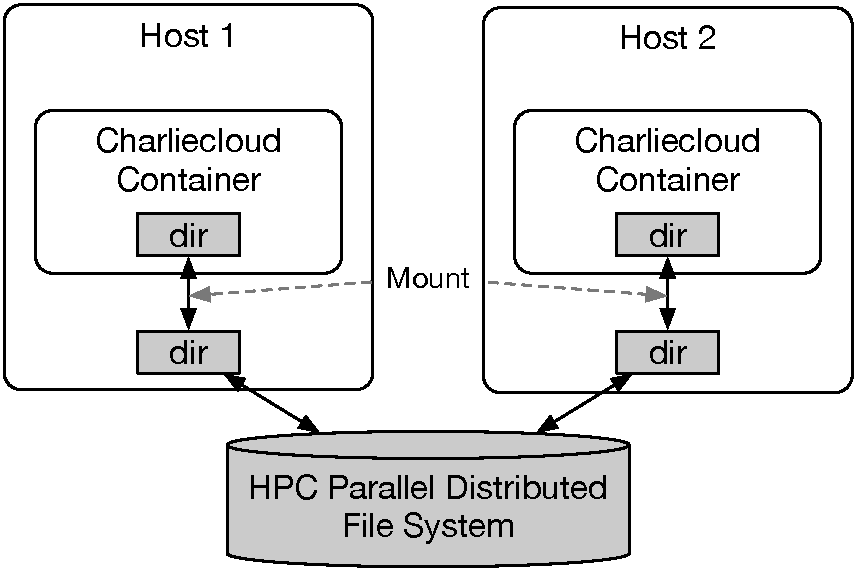
\includegraphics[width=0.4\textwidth]{figures/bee-cc.pdf}
    \caption{Shared Storage Design using Virtual IO}
    \label{bee-cc}
    \vspace*{-1em}
\end{figure}

When designing a \texttt{BEE backend}, one problem is identifying the suitable balance point between sharing and isolation of the runtime environment. Charliecloud offers comparable runtime isolation to Docker, that enables the user to pack all dependencies and tools in the image, avoiding additional application-specific configuration in the runtime environment. On the other hand, HPC applications usually require some degrees of data sharing: \textit{sharing via network} and \textit{sharing via storage}. 

\subsection{Network Design}
Sharing via network means processes running on different containers need to be able to share data via network. Charliecloud by default exposes all hardware network interfaces to its container runtime environment. Since HPC systems usually have interconnected networks between nodes, processes running in Charliecloud can communicate through the network interfaces on each node and get the benefits of any available network technology e.g., Infiniband. So, in \texttt{BEE-Charliecloud} we choose to the keep the default network settings. 

\subsection{Storage Design}
Sharing via storage is not natively supported by Charliecloud. By default each container only mounts the filesystem in the flattened input image. To enable sharing via storage, we use the \texttt{--bind} option  at container launch time to mount an user-specified host directory to a shared directory inside the container as mentioned in the user interface section. Since HPC systems usually have shared filesystem among nodes, processes can share data via the shared directory inside each container as shown in \textbf{Fig. \ref{bee-cc}} After each container is configured, \texttt{BEE-Charliecloud} automatically executes user's runscripts via the Charliecloud command \texttt{ch-run}. When initiating MPI parallel jobs, \texttt{BEE-Charliecloud} wraps \texttt{mpirun} command outside \texttt{ch-run} together with necessary MPI launching options. When deployed on HPC systems with Slurm resource manager, \texttt{BEE-Charliecloud} can interact with Slurm frontend to configure computing resources automatically. \textbf{Algorithm \ref{bee-cc-launch}} shows the launching logic of \texttt{BEE-Charliecloud}.

\begin{algorithm}
\caption{\texttt{BEE-Charliecloud} launching logic}
\label{bee-cc-launch}
\begin{algorithmic}[1]
\REQUIRE{Dockerized application (Docker image/Dockerfile)}
\REQUIRE{\texttt{BEE} configuration file (\texttt{beefile})}
\REQUIRE{Run scripts}
\STATE \texttt{pull/build\_docker(beefile)}
\STATE \texttt{flattened\_tar\_file $\leftarrow$ ch-docker2tar(docker\_image)}
\STATE \texttt{flattened\_filesystem $\leftarrow$ ch-tar2dir(flattened\_tar\_file)}
\STATE \texttt{compose\_ch-run\_options()}
\FOR{\textbf{each} \texttt{sequential run script} \textbf{in} \texttt{beefile} }
\STATE \texttt{slurm\_allocate\_resources()}
\STATE \texttt{ch-run(script)}
\ENDFOR
\FOR{\textbf{each} \texttt{parallel run script} \textbf{in} \texttt{beefile} }
\STATE \texttt{slurm\_allocate\_resources()}
\STATE \texttt{mpirun\_ch-run(mpi\_script)}
\ENDFOR

\end{algorithmic}
\end{algorithm}
\section{BEE-VM Design}
\label{bee-vm-section}
%As mentioned before, some older HPC systems still run Linux system with kernel version incompatible with Docker runtime or any customized runtime system. 

To support \texttt{BEE} on older HPC systems that do not have Linux user namespace enabled, we design a second \texttt{BEE backend} for HPC system - \texttt{BEE-VM}, so that together with \texttt{BEE-Charliecloud} they make \texttt{BEE} support majority of the current HPC systems.
\texttt{BEE-VM} creates a VM layer on top of the host and then deploys Docker on the VM layer; as shown in \textbf{Fig. \ref{bee-backend}}. VM brings the isolation that enables us to run Docker even on a system with constraint. It utilizes Kernel-based Virtual Machine (KVM) (on by default in Linux), a hardware accelerated hypervisor, to provide bare-metal performance. As shown in \textbf{Fig. \ref{bee-vm}}, we run one VM per HPC host node and one Docker container per VM.

%For machines without KVM, we build and configure Quick Emulator (QEMU) in user space. QEMU runs on many host operating systems and on Linux, since kernel 2.6, that makes \texttt{BEE-VM} compatible with almost all HPC machines; however, QEMU without paravirtualization does introduce a significant performance penalty.

Similar to \texttt{BEE-Charliecloud}, besides running applications in isolated environment, another goal of the \texttt{BEE-VM} design is enabling two kinds of sharing, \textit{sharing via network} and \textit{sharing via storage}, between Docker container applications running on different machines. 
 
\subsection{Network Design}
The network design of \texttt{BEE-VM} mainly targets two functions: (1) \texttt{BEE} needs to remotely login and control each VM via SSH; (2) MPI needs network to share data between processes. 
%The network design of \texttt{BEE-VM} mainly targets two functions: First, we need to dynamically configure and deploy our VM and Docker container. This needs to be done automatically and remotely by \texttt{BEE}. We choose to utilize SSH for remote configuration. Also, since we are aiming at HPC application and most HPC applications require MPI, we need to dynamically compose a network for MPI communication between different computing nodes. For enabling that, we create a virtual subnet comprised of all VMs and corresponding Docker containers, so that they can communicate with each other.

%\subsubsection{Inter-VM network}
%We first discuss the network design at the VM layer. This is necessary because the Docker container will rely on the VM's network configuration for network in the container. 

In order to enable the SSH connection to the VM through the host, the hypervisor is configured to create dedicated virtual network interface card (vNIC) used for port forwarding that maps an unused port on the host to the SSH port on the VM. As for MPI, it cannot use the vNIC for SSH, since it usually uses a different (random) port for communication, so we cannot use port forwarding on a specific port. To handle this problem, we have two solutions. For a system with regular Ethernet, we create a second vNIC on each VM and connect all of them in a virtual subnet (i.e., multicast or P2P connection). We choose this over more straight forward approaches  (e.g., bridging) because this approach does not require any administrative privilege to the system. For a system with InfiniBand, we adopt Single Root Input/Output Virtualization (SR-IOV) to connect all VMs. To connect all the Docker containers together, we choose to start the Docker container in 'host network' in which all network configurations are exposed to the container, so that each container has the same connectivity as VM.



\subsection{Storage Design}
%\subsubsection{VM layer}
To share data between processes in Docker containers, we need to first build a shared filesystem between different VMs. Here, we use the Virtio feature \cite{russell2008virtio} in QEMU to map a host directory to a directory inside VMs. It only requires minimum configuration at VM boot time. Since HPC systems usually use shared filesystem (via NFS, Luster, etc.), each VM will also have the same file-sharing capability as long as they map to the same host directory. For data sharing in the Docker layer, we use the data volume mount feature in Docker to mount the shared folder inside VM to a directory in Docker. Since Docker runs as a process at the VM layer, mounting the data volume adds negligible overhead. 

%Since it does not rely on the virtual network, the whole virtual network is saved for MPI.

\begin{figure}[h]
	%\vspace*{-1em}
    \centering
    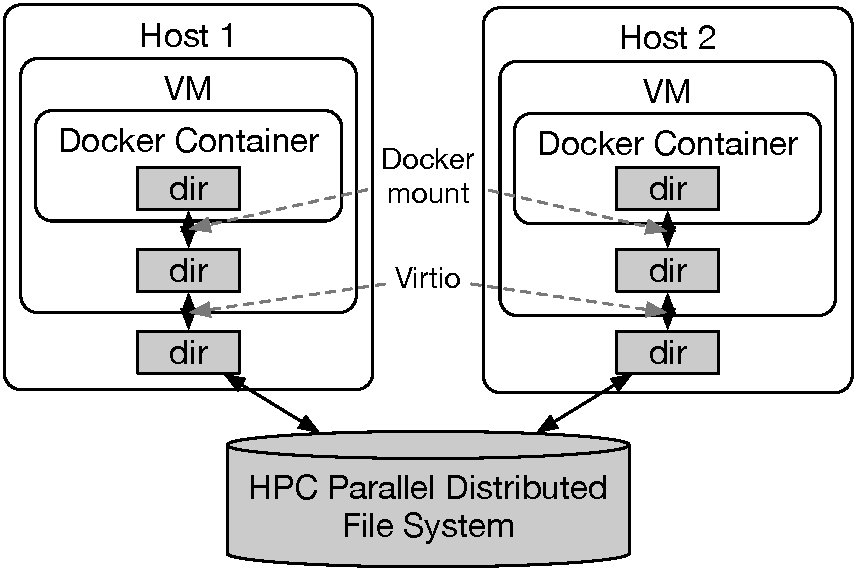
\includegraphics[width=0.4\textwidth]{figures/virtio.pdf}
    \caption{Shared Storage Design using Virtual IO}
    \label{bee-vm}
    \vspace*{-1em}
\end{figure}

%\subsubsection{Docker container layer}



\subsection{BEE-VM Deployment}
\textbf{Algorithm \ref{bee-launch}} shows the launching logic of \texttt{BEE-VM}. Before using \texttt{BEE-VM} the first time, users need to use the image builder provided by \texttt{BEE} to build the base VM image. The image is customized for \texttt{BEE-VM} that includes pre-installed softwares and settings. It only need to be done once. After that each VM will only work on a copy of the base image without any modification to the base image. During launch, \texttt{BEE-VM} first deploys VM on each HPC node (line 1 - 6). Next, the hostfile on each VM is setup in order to let each VM communicate with each other without using complicated IP addresses. The virtio storage is mounted in line 14. In the next stage, depending on what the user provides, \texttt{BEE-VM} will either pull the Docker image from public/private registries or build a new Docker image from a Dockerfile loaded into the local VM. Finally, \texttt{BEE} starts the application by launching from the first node (i.e., master node).


\begin{algorithm}
\caption{\texttt{BEE-VM} launching logic}
\label{bee-launch}
\begin{algorithmic}[1]
\REQUIRE{Pre-built QEMU Img. (only need to build once)}
\REQUIRE{Allocated host nodes: $H_1$, $H_2$,..., $H_k$}
\REQUIRE{Dockerized application (Docker image/Dockerfile)}
\REQUIRE{\texttt{BEE} configuration file (\texttt{beefile})}
\REQUIRE{Run scripts}

\FOR{i \textbf{in} 1 \textbf{to} \texttt{beefile}.num\_of\_nodes}
	\STATE \texttt{node\_i.copy\_img()}
	\STATE \texttt{node\_i.compose\_qemu\_arg(storage\_dir)}
	\STATE \texttt{node\_i.compose\_qemu\_arg(network\_conf)}
    \STATE \texttt{node\_i.start\_vm()}
\ENDFOR
\STATE \texttt{wait\_for\_all\_vm\_to\_become\_ready()}
\FOR{i in 1 \textbf{to} \texttt{beefile}.num\_of\_nodes}
\STATE \texttt{node\_i.set\_hostname()}
\FOR{j in 1 \textbf{to} \texttt{beefile}.num\_of\_nodes}
\STATE \texttt{node\_j.setup\_hostfile(node\_i.ip())}
\ENDFOR
\ENDFOR
\FOR{i in 1 \textbf{to} \texttt{beefile}.num\_of\_nodes}
\STATE \texttt{node\_i.mount\_via\_virtio()}
\ENDFOR
\FOR{i in 1 \textbf{to} \texttt{beefile}.num\_of\_nodes}
\STATE \texttt{node\_i.pull/build\_docker(beefile)}
\STATE 
\texttt{node\_i.conf\_docker\_storage(efs\_mnt)}
\STATE \texttt{node\_i.conf\_docker\_network(host\_mode)}
\STATE \texttt{node\_i.start\_docker('ssh daemon')}
\ENDFOR
\FOR{\textbf{each} \texttt{sequential run script} \textbf{in} \texttt{beefile} }
\STATE \texttt{node\_0.docker\_exec(script)}
\ENDFOR
\FOR{\textbf{each} \texttt{parallel run script} \textbf{in} \texttt{beefile} }
\STATE \texttt{node\_0.docker\_exec(mpi\_script)}
\ENDFOR

\end{algorithmic}
\end{algorithm}

\section{BEE-AWS Design}
\label{bee-aws-section}
AWS is one of the most widely used commercial cloud computing platforms. It offers great configuration flexibility towards computing software/hardware environment, network, storage, and security. Many researchers from both HPC and cloud community use AWS to run large scale applications. However, configuring the desired computing environment on AWS is tedious and can impede experiment workflow, especially for users with less knowledge or experience on AWS. Although many tools offer the ability to automate the computing environment setup process, they usually cannot create an environment suitable for HPC applications. Even though tools such as StarCluster \cite{starcluster}, do offer the capability of creating HPC-friendly environment on AWS, it suffers from two drawbacks. First, they do not offer the support of automatic Docker container deployment and execution. Users still need to manually deploy and run their applications. Second, they usually do not offer HPC/cloud cross-platform support. %Users need to seek for other tools for other platforms. 

Here we design \texttt{BEE-AWS} as another \texttt{BEE backend}. \texttt{BEE-AWS} enables the same end-to-end automation on AWS as provided in \texttt{BEE-Charliecloud} and \texttt{BEE-VM} on HPC systems. Most importantly, \texttt{BEE-AWS} offers the same user interface and execution environment as \texttt{BEE-VM}, so the user only needs to make minimum modifications to the \texttt{BEE} configuration file (\texttt{beefile}) in order to switch to AWS. 

The computing resources are based on Xen-based VMs and they also known as EC2 instances. Since EC2 instances are VM-based, users are given full control inside each VM. So, here we configure them (via customized AMI) to enable Docker runtime. Users of \texttt{BEE} can specify desired instance type via \texttt{BEE} configuration file (\texttt{beefile}). Same as on the HPC platform, data sharing via network and storage also need to be handled.

\subsection{Network Design}
EC2 instances by default have network interconnect capability via the network in their infrastructures. However, they still need to be customized for HPC applications. First, as mentioned in \texttt{BEE-VM} design, MPI commonly uses random port for communication, so we need to create an EC2 security group that has a range of ports opened based on the MPI implementation specification. Second, for fast network interconnection, EC2 instances need to be placed in the same placement group. This makes sure the physical hardware allocated for each EC2 instance are close to each other so that the network is optimized for low latency and high throughput. As for network interconnection between Docker containers, we follow a similar choice made using \texttt{BEE-VM}, that enables 'host network' mode at launch time.

\subsection{Storage Design}
By default EC2 instances do not share filesystems. To enable file sharing, we choose to create Elastic File System (EFS) and mount EFS to each EC2 instance. This design has better performance than the master-slave based Network File System (NFS) adopted in Starcluster. We use the volume mounting feature of Docker to enable file sharing between Docker containers similar to \texttt{BEE-VM}.

\textbf{Algorithm \ref{bee-aws-launch}} shows that launching logic of \texttt{BEE-AWS}. We use Boto API to remotely launch EC2 instances on AWS (line 7 - 15). After that we use SSH connection to control each instance. 

\begin{algorithm}
\caption{\texttt{BEE-AWS} launching logic}
\label{bee-aws-launch}
\begin{algorithmic}[1]
\REQUIRE{Pre-built AMI (only need to build once)}
\REQUIRE{Dockerized application (Docker image/Dockerfile)}
\REQUIRE{\texttt{BEE} configuration file (\texttt{beefile})}
\REQUIRE{Run scripts}
\IF {\textit{user given EFS name} not exist}
\STATE \texttt{request\_creating\_efs(efs\_name)}
\WHILE{ \texttt{efs\_status(efs\_name)} != \texttt{active}}
\STATE \texttt{sleep()}
\ENDWHILE
\ENDIF

\STATE \texttt{initialize\_ec2\_service\_connection()}
\STATE \texttt{bee\_sg = create\_security\_group()}
\STATE \texttt{bee\_sg.authroize\_ingress('tcp', '22')}
\STATE \texttt{bee\_pg = create\_placement\_group()}
\FOR{i in 1 \textbf{to} \texttt{beefile}.num\_of\_nodes}
\STATE \texttt{bee\_ec2\_i = create\_ec2(bee\_sg, bee\_pg)}
\STATE \texttt{bee\_ec2\_i.start()}
\ENDFOR
\STATE \texttt{wait\_for\_all\_instance\_to\_become\_ready()}
\FOR{i in 1 \textbf{to} \texttt{beefile}.num\_of\_nodes}
\STATE \texttt{bee\_ec2\_i.set\_hostname()}
\FOR{j in 1 \textbf{to} \texttt{beefile}.num\_of\_nodes}
\STATE \texttt{bee\_ec2\_j.setup\_hostfile(bee\_ec2\_i.ip)}
\ENDFOR
\ENDFOR
\FOR{i in 1 \textbf{to} \texttt{beefile}.num\_of\_nodes}
\STATE \texttt{bee\_ec2\_i.create\_efs\_mount\_point()}
\STATE \texttt{bee\_ec2\_i.mount\_to\_efs(efs\_name)}
\STATE \texttt{bee\_ec2\_i.pull/build\_docker(beefile)}
\ENDFOR
\FOR{i in 1 \textbf{to} \texttt{beefile}.num\_of\_nodes}
\STATE \texttt{bee\_ec2\_i.pull/build\_docker(beefile)}
\STATE \texttt{bee\_ec2\_i.conf\_docker\_storage(efs\_mnt)}
\STATE \texttt{bee\_ec2\_i.conf\_docker\_network(host\_mode)}
\STATE \texttt{bee\_ec2\_i.start\_docker('ssh daemon')}
\ENDFOR
\FOR{\textbf{each} \texttt{sequential run script} \textbf{in} \texttt{beefile} }
\STATE \texttt{bee\_ec2\_0.docker\_exec(script)}
\ENDFOR
\FOR{\textbf{each} \texttt{parallel run script} \textbf{in} \texttt{beefile} }
\STATE \texttt{bee\_ec2\_0.docker\_exec(mpi\_script)}
\ENDFOR
\end{algorithmic}
\end{algorithm}

%\section{BEE-AWS Design}
%AWS is a highly usable computing environment for cloud and HPC users. To provide a similar Docker-enabled environment on AWS, we designed another back-end \texttt{BEE}, the \texttt{BEE-AWS}. It enables the user to run their Dockerized application on AWS using \texttt{BEE-AWS} the same way as they run on the HPC system using \texttt{BEE-VM}. Since both the storage and network on AWS are highly optimized and their configurations are hidden from users, the design of \texttt{BEE-AWS} is relatively simpler than \texttt{BEE-VM}. In \texttt{BEE-AWS}, it first launches an AWS instance based cluster using BOTO API \cite{BOTOAPI} with optimized network configuration and a shared EFS storage. Then, it loads the user application's input data into EFS for storage sharing. Next, \texttt{BEE-AWS} controls each instance to obtain Docker images either from public/private docker registries or builds Docker images from Dockerfiles. Finally, it starts the user application in Docker containers.
\section{BEE-OpenStack Design}
\label{bee-openstack-section}
OpenStack is a cloud operating system that is able to manage large pools of computing, storage, and network resources. It has been widely deployed in both research facilities and cloud computing environments. To bring the same unified execution environment and end-to-end automation to OpenStack, we build \texttt{BEE-OpenStack} as another \texttt{BEE backend}.

Unlike AWS, the computing sources of OpenStack can be either bare-metal machines or VM. In either case, users are given full control inside the operating system. So, similar to \texttt{BEE-AWS} we enable Docker runtime inside each OpenStack instance. 

\subsection{Network Design}
On our OpenStack test environment (\texttt{Chameleon Cloud}), network interconnects are enabled by default between instances. So, we do not need to further configure it. For OpenStack infrastructures that need customized network, \texttt{BEE} will configure it automatically to ensure network interconnect capabilities between instances. The detail is omitted here. Similar to before, we use 'host network' mode for Docker containers.

\subsection{Storage Design}
Similar to \texttt{AWS}, by default, OpenStack instances do not share filesystems. On our OpenStack test environment (\texttt{Chameleon Cloud}), there is no OpenStack-managed storage system. So, we adopt NFS based file sharing between master instance (first instance) and worker instances. We use the volume mounting feature of Docker to enable file sharing between Docker containers similar to \texttt{BEE-VM} and \texttt{BEE-AWS}

\textbf{Algorithm \ref{bee-openstack}} shows the launching logic of \texttt{BEE-OpenStack}. Here we first use OpenStack CLI client to launch a pre-built Stack template for BEE, and then use SSH to control each instance.

\begin{algorithm}
\caption{\texttt{BEE-OpenStack} launching logic}
\label{bee-openstack}
\begin{algorithmic}[1]
\REQUIRE{Pre-built OpenStack Img. (only need to build once)}
\REQUIRE{Dockerized application (Docker image/Dockerfile)}
\REQUIRE{\texttt{BEE} configuration file (\texttt{beefile})}
\REQUIRE{Run scripts}
\STATE \texttt{initialize\_nova\_service\_connection()}
\STATE \texttt{create\_new\_sshkey()}
\STATE \texttt{launch\_bee\_stack(\texttt{beefile})}
\STATE \texttt{wait\_for\_all\_instance\_to\_become\_ready()}

\FOR{i in 1 \textbf{to} \texttt{beefile}.num\_of\_nodes}
\STATE \texttt{bee\_os\_i.set\_hostname()}
\FOR{j in 1 \textbf{to} \texttt{beefile}.num\_of\_nodes}
\STATE \texttt{bee\_os\_j.setup\_hostfile(bee\_os\_i.ip)}
\ENDFOR
\ENDFOR
\STATE \texttt{bee\_os\_0.create\_nfs\_mount\_point()}
\FOR{i in 1 \textbf{to} \texttt{beefile}.num\_of\_nodes}
\STATE \texttt{bee\_os\_i.mount\_to\_nfs(bee\_os\_0.ip())}
\ENDFOR
\FOR{i in 1 \textbf{to} \texttt{beefile}.num\_of\_nodes}
\STATE \texttt{bee\_os\_i.pull/build\_docker(beefile)}
\ENDFOR
\FOR{i in 1 \textbf{to} \texttt{beefile}.num\_of\_nodes}
\STATE \texttt{bee\_os\_i.pull/build\_docker(beefile)}
\STATE \texttt{bee\_os\_i.conf\_docker\_storage(nfs\_mnt)}
\STATE \texttt{bee\_os\_i.conf\_docker\_network(host\_mode)}
\STATE \texttt{bee\_os\_i.start\_docker('ssh daemon')}
\ENDFOR
\FOR{\textbf{each} \texttt{sequential run script} \textbf{in} \texttt{beefile} }
\STATE \texttt{bee\_os\_0.docker\_exec(script)}
\ENDFOR
\FOR{\textbf{each} \texttt{parallel run script} \textbf{in} \texttt{beefile} }
\STATE \texttt{bee\_os\_0.docker\_exec(mpi\_script)}
\ENDFOR
\end{algorithmic}
\end{algorithm}
\section{Evaluation}
\label{evaluation-section}
We evaluate the four \texttt{BEE backends} on four different platforms: For \texttt{BEE-Charliecloud}
%, we use our testbed cluster system Darwin. Each node has two 8-core Intel Ivy Bridge E5-2650 v2 CPUs with 251GB RAM. For
and \texttt{BEE-VM}, we test them on the bare-metal envionment on \texttt{Chameleon Cloud} at Texas Advanced Computing Center (TACC). Each node is equipped with two Intel Xeon E5-2670 v3 CPU (clock frequency at 2.30 GHz) with 128 GB DRAM. Each node is connected with Mellanox ConnectX-3 Infiniband card with peak transfer speed at 10 Gbps.  For \texttt{BEE-AWS}, we choose to use \texttt{c3.4xlarge} EC2 type at AWS Oregon region. Each node is equipped with Intel Xeon E5-2680 v2 CPUs and 30GB DRAM. On \texttt{BEE-OpenStack}, we choose the OpenStack environment at \texttt{Chameleon Cloud}@University of Chicago. We focus on evaluating three kinds of performance that are most important for HPC applications: \textit{computation}, \textit{storage}, and \textit{network}. For each test, the comparison baseline is the native performance provided on each platform without using \texttt{BEE} or any additional encapsulated runtime system. Note: all platforms, except AWS, provide access to the bare-metal hardware, so baseline performance is the native performance on the hardware. For AWS, its Xen-based VM is an inseparable part of the platform and the underlying physical hardware is inaccessible to general users, so its baseline is the performance inside VMs.

\begin{figure*}[t]
    \centering
    \begin{subfigure}[t]{0.49\textwidth}
        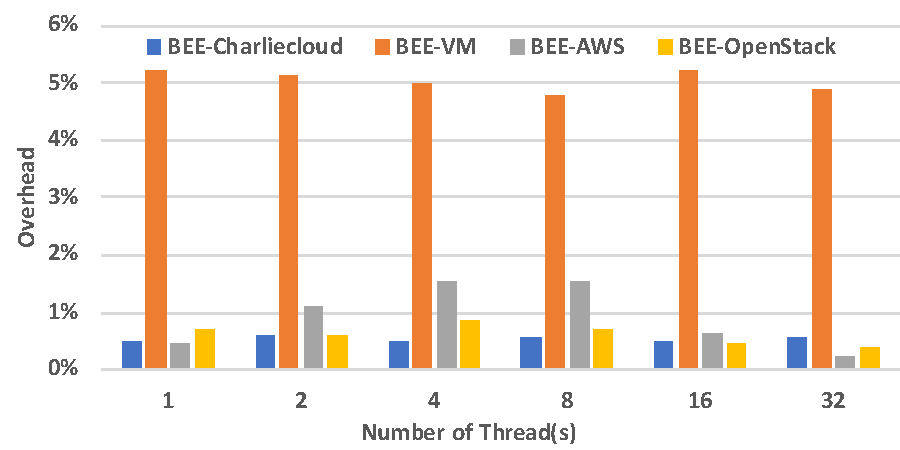
\includegraphics[width=\textwidth]{figures/bt.pdf}
        \caption{Compute intensive workload (BT)}
    \end{subfigure}
    \begin{subfigure}[t]{0.49\textwidth}
        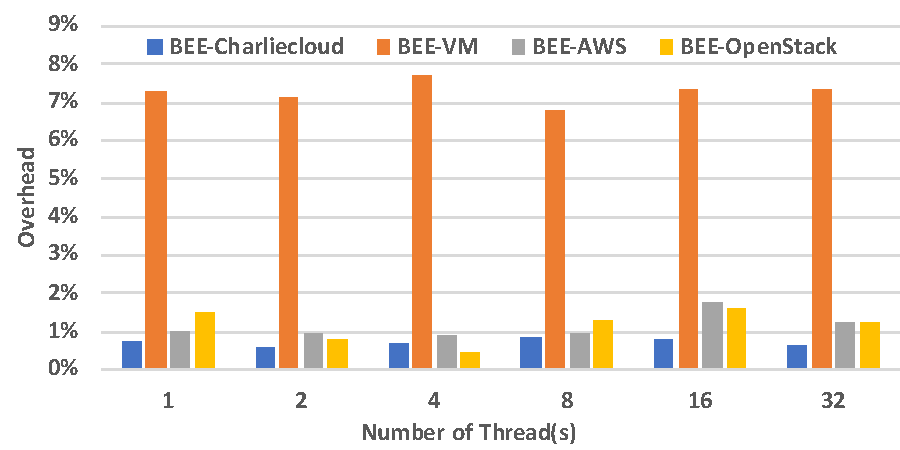
\includegraphics[width=\textwidth]{figures/is.pdf}
        \caption{Memory intensive workload (IS)}
    \end{subfigure}
    \vspace*{-0.5em}
    \caption{Performance overhead compare with native performance provided on each corresponding platform.}
    \label{comp}
    \vspace*{-1em}
\end{figure*}

\begin{figure*}[t]
    \centering
    \begin{subfigure}[t]{0.49\textwidth}
        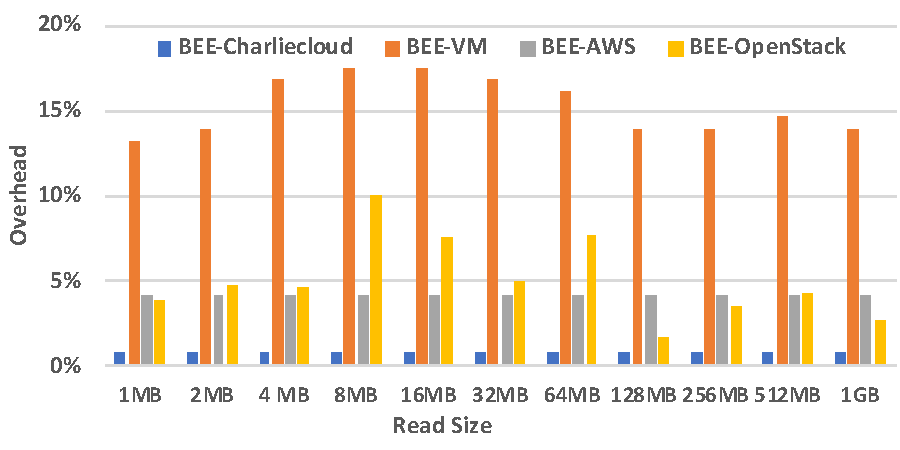
\includegraphics[width=\textwidth]{figures/read.pdf}
        %\caption{Compute intensive workload (BT)}
    \end{subfigure}
    \begin{subfigure}[t]{0.49\textwidth}
        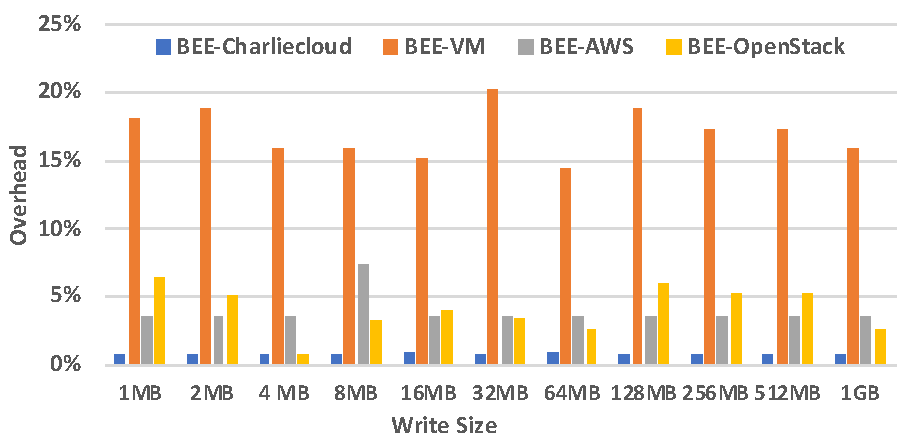
\includegraphics[width=\textwidth]{figures/write.pdf}
        %\caption{Memory intensive workload (IS)}
    \end{subfigure}
    \vspace*{-0.5em}
    \caption{Storage I/O read/write speed overhead compare with native speed provided on each corresponding platform.}
    \label{io}
    \vspace*{-2em}
\end{figure*}



\subsection{Computational Performance}
Computational performance of a platform is one of the most important capabilities for HPC applications. In this section, we compare the computational performance of all four \texttt{BEE backends} with the baseline. We choose one compute intensive benchmark test and one memory intensive benchmark test from the OpenMP version NAS Parallel Benchmarks (NPB)\cite{npb} in our evaluation. We test each benchmark running one to 32 threads (cores) to further show the computational performance on multi-thread environment. 
\subsubsection{Compute intensive workload}
For compute intensive workload, we choose Block Tri-diagonal solver (BT) benchmark test with input matrix size of $102^3$ (problem size: \texttt{class B}).

\begin{comment}
\begin{figure}[t]
    \centering
    \begin{subfigure}[t]{0.24\textwidth}
        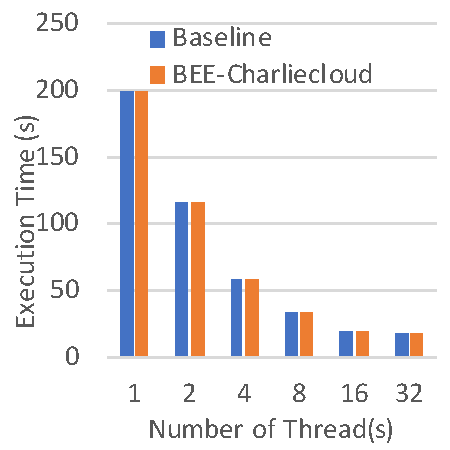
\includegraphics[width=\textwidth]{figures/bt-bee-cc.pdf}
        \caption{\texttt{BEE-Charliecloud}}
    \end{subfigure}
    \begin{subfigure}[t]{0.24\textwidth}
        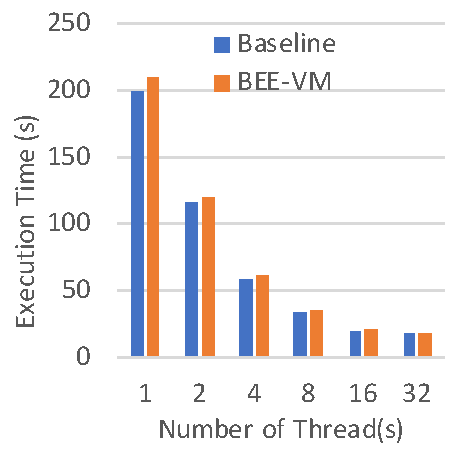
\includegraphics[width=\textwidth]{figures/bt-bee-vm.pdf}
        \caption{\texttt{BEE-VM}}
    \end{subfigure}
    \begin{subfigure}[t]{0.24\textwidth}
        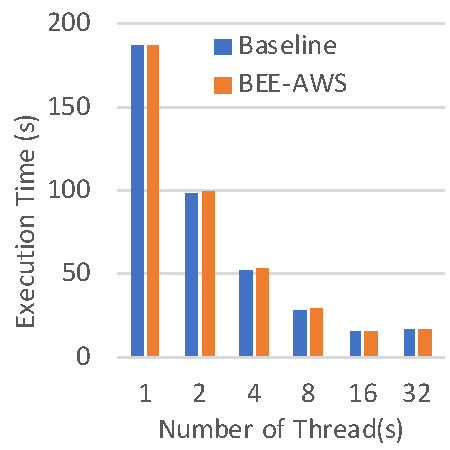
\includegraphics[width=\textwidth]{figures/bt-bee-aws.pdf}
        \caption{\texttt{BEE-AWS}}
    \end{subfigure}
    \begin{subfigure}[t]{0.24\textwidth}
        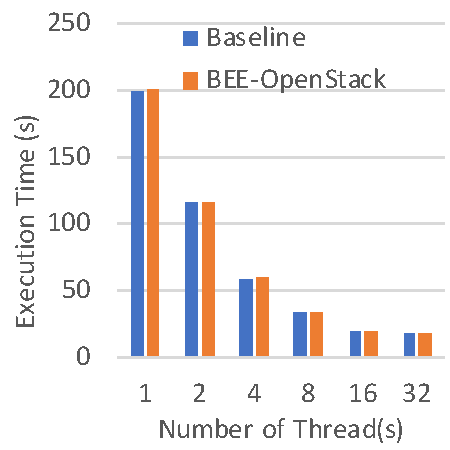
\includegraphics[width=\textwidth]{figures/bt-bee-os.pdf}
        \caption{\texttt{BEE-OpenStack}}
    \end{subfigure}
    %\vspace*{-0.5em}
    \caption{Performance comparison on compute intensive workload (BT).}
    \label{comp}
    %\vspace*{-2em}
\end{figure}
\end{comment}



As we can see in \textbf{Fig. \ref{comp}(a)}, for compute intensive workload, all four \texttt{BEE backends} have low performance overhead: \texttt{BEE-Charliecloud} 0.4\% - 0.6\% (avg. 0.5\%); \texttt{BEE-VM} 4.8\% - 5.2\% (avg. 5.0\%); \texttt{BEE-AWS} 0.2\% - 1.6\% (avg. 0.8\%); \texttt{BEE-OpenStack} 0.3\% - 0.9\% (avg. 0.6\%).
    
\subsubsection{Memory intensive workload}
For memory intensive workload, we choose Integer Sort  (IS) test suit with 134217728 input integer (problem size : \texttt{class C}). 

\begin{comment}


\begin{figure}[t]
    \centering
    \begin{subfigure}[t]{0.24\textwidth}
        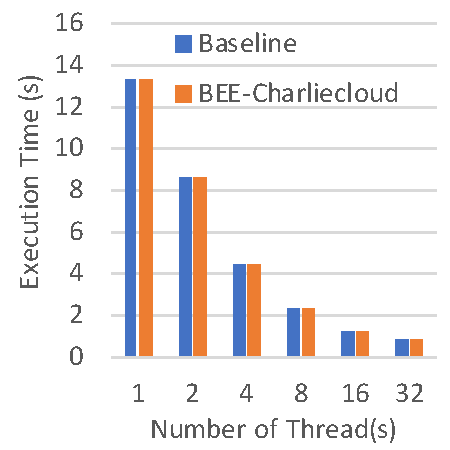
\includegraphics[width=\textwidth]{figures/is-bee-cc.pdf}
        \caption{\texttt{BEE-Charliecloud}}
    \end{subfigure}
    \begin{subfigure}[t]{0.24\textwidth}
        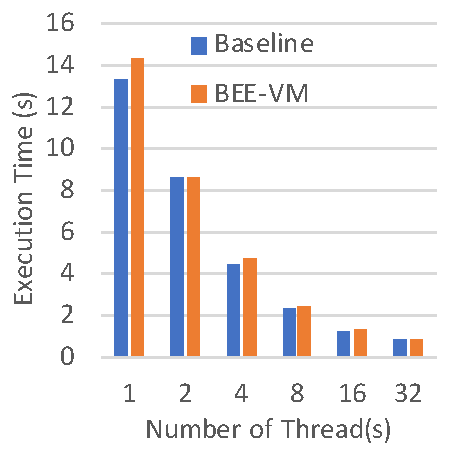
\includegraphics[width=\textwidth]{figures/is-bee-vm.pdf}
        \caption{\texttt{BEE-VM}}
    \end{subfigure}
    \begin{subfigure}[t]{0.24\textwidth}
        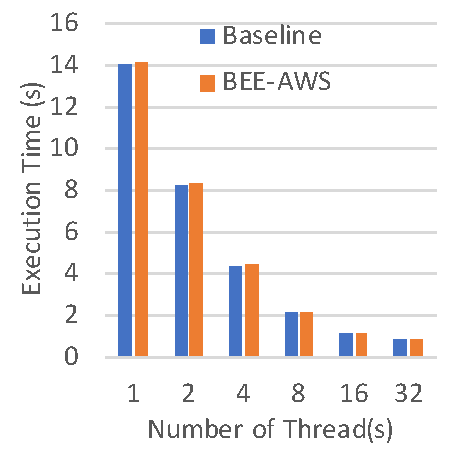
\includegraphics[width=\textwidth]{figures/is-bee-aws.pdf}
        \caption{\texttt{BEE-AWS}}
    \end{subfigure}
    \begin{subfigure}[t]{0.24\textwidth}
        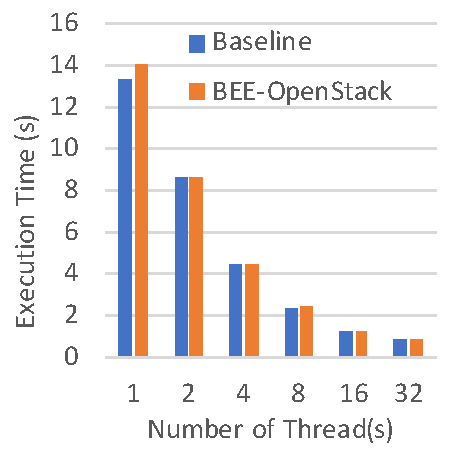
\includegraphics[width=\textwidth]{figures/is-bee-os.pdf}
        \caption{\texttt{BEE-OpenStack}}
    \end{subfigure}
    %\vspace*{-0.5em}
    \caption{Performance comparison on memory intensive workload (IS).}
    \label{mem}
   % \vspace*{-2em}
\end{figure}
\end{comment}


As we can see in \textbf{Fig. \ref{comp}(b)}, for memory intensive workload all four \texttt{BEE backends} also have low performance overhead: \texttt{BEE-Charliecloud} 0.6\% - 0.9\% (avg. 0.7\%); \texttt{BEE-VM} 6.9\% - 7.7\% (avg. 7.1\%); \texttt{BEE-AWS} 0.9\% - 1.8\% (avg. 1.1\%); \texttt{BEE-OpenStack} 0.5\% - 1.7\% (avg. 1.0\%). In addition, both kinds of workload also exhibit similar speedup comparing with their baseline counterparts when we increase the number of threads.

 \begin{figure*}[t]
    \centering
    \begin{subfigure}[t]{0.245\textwidth}
        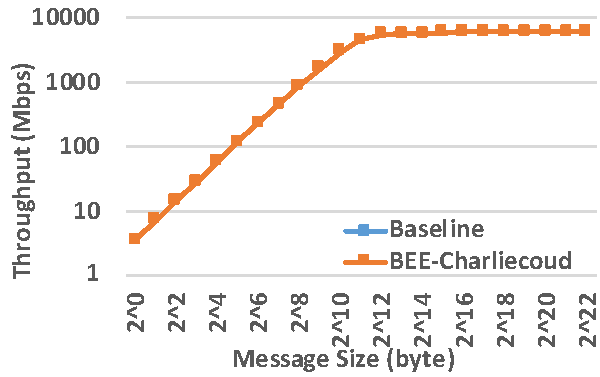
\includegraphics[width=\textwidth]{figures/band-bee-cc.pdf}
    \end{subfigure}
    \begin{subfigure}[t]{0.245\textwidth}
        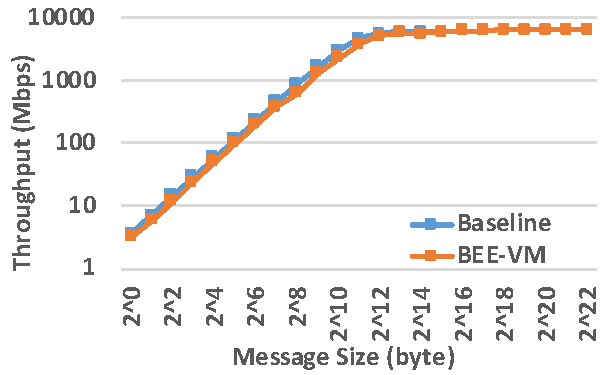
\includegraphics[width=\textwidth]{figures/band-bee-vm.pdf}
    \end{subfigure}
    \begin{subfigure}[t]{0.245\textwidth}
        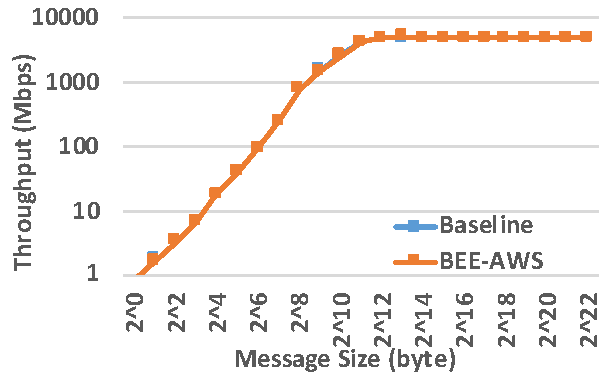
\includegraphics[width=\textwidth]{figures/band-bee-aws.pdf}
    \end{subfigure}
    \begin{subfigure}[t]{0.245\textwidth}
        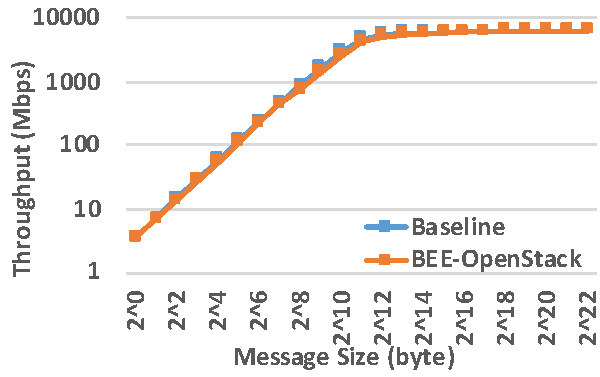
\includegraphics[width=\textwidth]{figures/band-bee-os.pdf}
    \end{subfigure}
    \caption{P2P Network Throughput Comparison}
    \label{net-band}
   % \vspace*{-2em}
\end{figure*}
\begin{figure*}[t]
    \centering
    \begin{subfigure}[t]{0.245\textwidth}
        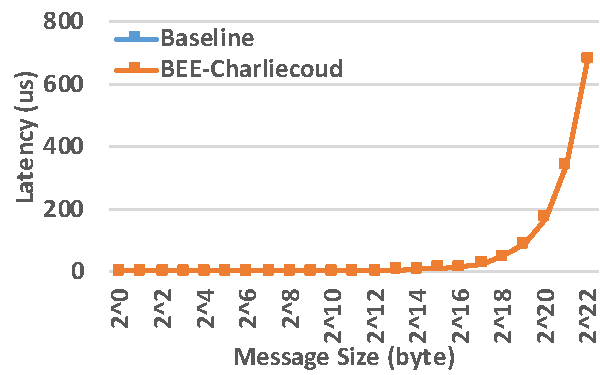
\includegraphics[width=\textwidth]{figures/lat-bee-cc.pdf}
    \end{subfigure}
    \begin{subfigure}[t]{0.245\textwidth}
        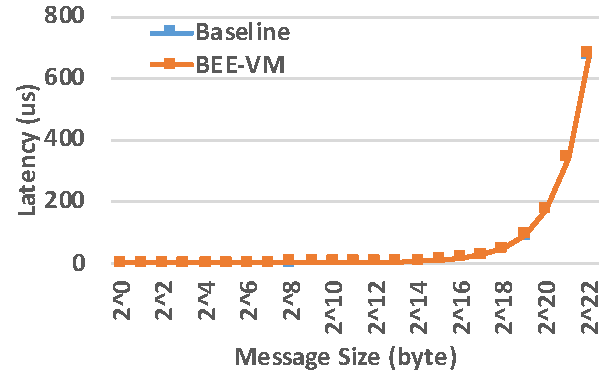
\includegraphics[width=\textwidth]{figures/lat-bee-vm.pdf}
    \end{subfigure}
    \begin{subfigure}[t]{0.245\textwidth}
        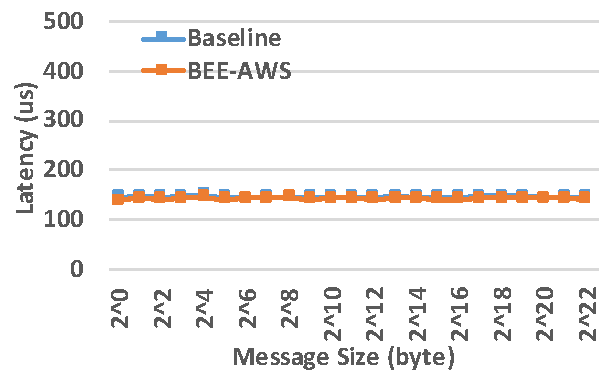
\includegraphics[width=\textwidth]{figures/lat-bee-aws.pdf}
    \end{subfigure}
    \begin{subfigure}[t]{0.245\textwidth}
        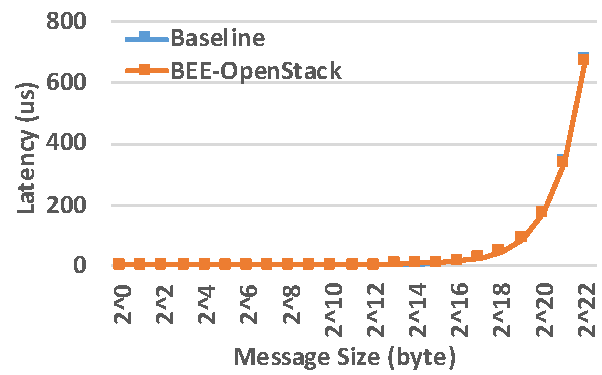
\includegraphics[width=\textwidth]{figures/lat-bee-os.pdf}
    \end{subfigure}
    \caption{P2P Network Latency Comparison}
    \label{net-lat}
   % \vspace*{-2em}
\end{figure*}

\begin{figure*}[t]
    \centering
    \begin{subfigure}[t]{0.245\textwidth}
        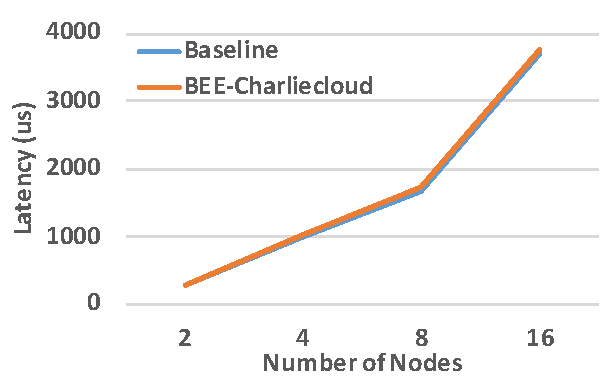
\includegraphics[width=\textwidth]{figures/cl-bee-cc.pdf}
    \end{subfigure}
    \begin{subfigure}[t]{0.245\textwidth}
        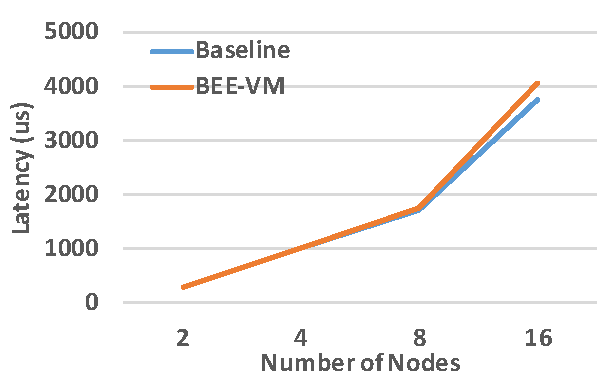
\includegraphics[width=\textwidth]{figures/cl-bee-vm.pdf}
    \end{subfigure}
    \begin{subfigure}[t]{0.245\textwidth}
        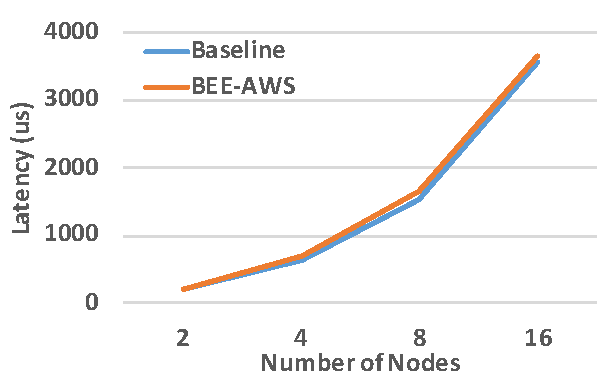
\includegraphics[width=\textwidth]{figures/cl-bee-aws.pdf}
    \end{subfigure}
    \begin{subfigure}[t]{0.245\textwidth}
        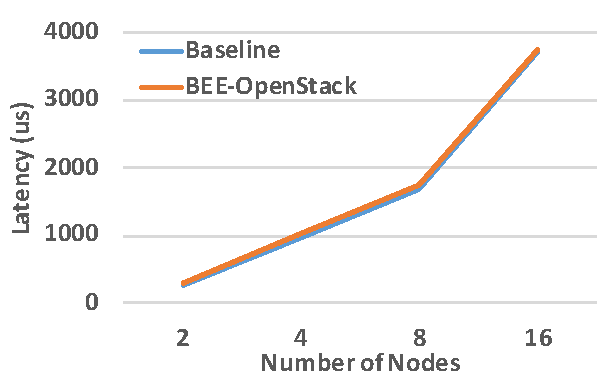
\includegraphics[width=\textwidth]{figures/cl-bee-os.pdf}
    \end{subfigure}
    \caption{All-to-all Network Latency Comparison}
    \label{net-lat-all}
    \vspace*{-2em}
\end{figure*}
\subsection{Storage I/O }
Storage I/O is another key component for many HPC applications. For example, large-scale simulations often need to first load large datasets before computation and frequently dump checkpoints during computation and once the simulation has concluded. Later, these results may be used for other simulations or for analytics. I/O performance plays an important role for the overall performance of HPC applications. 

To evaluate the storage I/O performance of the four \texttt{BEE backends} and compare with the baseline performance, we use the Linux built-in command -- \texttt{dd}. Specifically, to benchmark write performance, we use the \texttt{dd} command to write a file with data from \texttt{/dev/zero}. As for read performance, we use the \texttt{dd} command to read out the file just saved and write to \texttt{/dev/null}. To avoid reading from cache, we use \texttt{echo 3 > /proc/sys/vm/drop\_caches} command to force the system to clear all cached data between each write and read. Usually this file is read-only inside a container, so we issue the command outside the container, achieving the same cache flushing effect. The file used for write and read is placed in the directory that is shared between instances or containers. We test different file sizes ranging from 1 MB to 1 GB. To eliminate noise and variation, we repeat each test 1000 times. \textbf{Fig. \ref{io}} shows the read and write performance on the four \texttt{BEE backends} comparing with the baseline (i.e., the IO performance on each platform without using \texttt{BEE}). As we can see, \texttt{BEE-Charliecloud} produces negligible read and write overhead (~0.08\%). \texttt{BEE-VM} uses both VM and Docker, so it produces relative higher overhead, 13.1\% - 17.5\% (avg. 15.2\%) for read and 15.1\% - 20.1\% (avg. 17.1\%) for write. \texttt{BEE-AWS} produces steady 0.4\% overhead for read and 0.3\% overhead for write. \texttt{BEE-OpenStack} produces 1.7\% - 7.6\% (avg. 5.0\%) for read overhead and 2.7\% - 6.4\% (avg. 4.1\%) for write overhead.

\subsection{Network}
Finally, we evaluate the network performance of the four \texttt{BEE backends}. We use the HPCBench \cite{hpcbench} to measure the bandwidth and latency when transferring data of different sizes between two processes in containers or on the platform without using \texttt{BEE}. \texttt{BEE-VM} and \texttt{BEE-OpenStack} use the Infiniband (IB) on \texttt{Chameleon Cloud} via SR-IOV. \texttt{BEE-Charliecloud} and \texttt{BEE-AWS} use the Ethernet connection. \textbf{Fig. \ref{net-band}} and \textbf{Fig. \ref{net-lat}} show the point-to-point (P2P) network performance. MPI communication function calls between two nodes (one process per node) were used to test the average throughput and latency when transferring different message sizes. It can be seen that all four \texttt{BEE backends} can provide similar network bandwidth and latency compared to the baseline. \textbf{Fig. \ref{net-lat-all}} also show the latencies of all-to-all collective communication in MPI. It shows that all four \texttt{BEE backends} still provide similar network performance large scale. 

%It also shows promising trends on larger clusters. Similar results have been seen in \cite{zhang2016performance}. Note that the Docker container is slightly better than bare-metal in some cases due to the tuning difference under the test scenario.  


\begin{comment}


\begin{figure}[t]
    \centering
    \begin{subfigure}[t]{0.5\textwidth}
        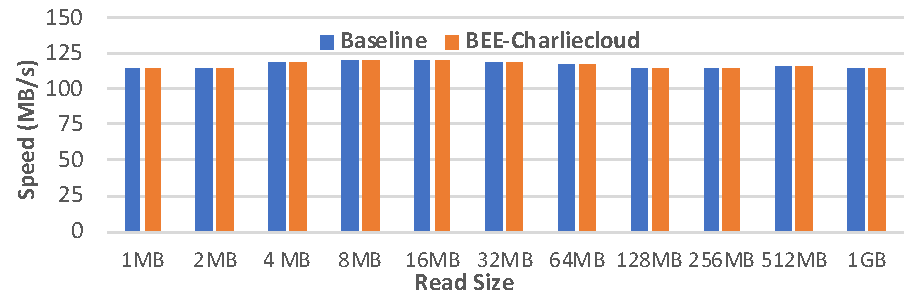
\includegraphics[width=\textwidth]{figures/read-bee-cc.pdf}
        \caption{Read Performance}
    \end{subfigure}
    \begin{subfigure}[t]{0.5\textwidth}
        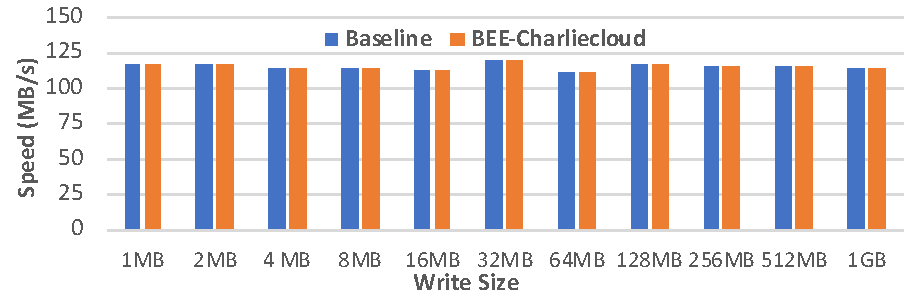
\includegraphics[width=\textwidth]{figures/write-bee-cc.pdf}
        \caption{Write Performance}
    \end{subfigure}
    %\vspace*{-0.5em}
    \caption{Comparison of storage I/O (\texttt{BEE-Charliecloud}).}
    \label{io-cc}
    \vspace*{-0em}
\end{figure}

\begin{figure}[t]
    \centering
    \begin{subfigure}[t]{0.5\textwidth}
        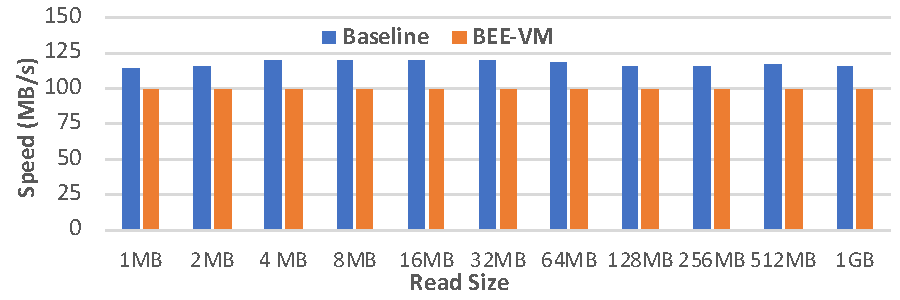
\includegraphics[width=\textwidth]{figures/read-bee-vm.pdf}
        \caption{Read Performance}
    \end{subfigure}
    \begin{subfigure}[t]{0.5\textwidth}
        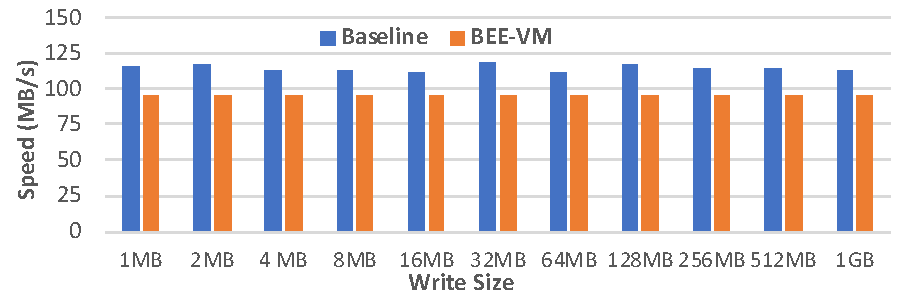
\includegraphics[width=\textwidth]{figures/write-bee-vm.pdf}
        \caption{Write Performance}
    \end{subfigure}
    %\vspace*{-0.5em}
    \caption{Comparison of storage I/O (\texttt{BEE-VM}).}
    \label{io-vm}
   \vspace*{-2em}
\end{figure}

\begin{figure}[t]
    \centering
    \begin{subfigure}[t]{0.5\textwidth}
        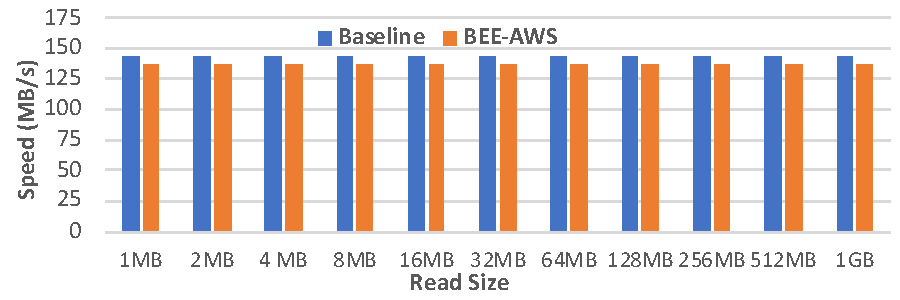
\includegraphics[width=\textwidth]{figures/read-bee-aws.pdf}
        \caption{Read Performance}
    \end{subfigure}
    \begin{subfigure}[t]{0.5\textwidth}
        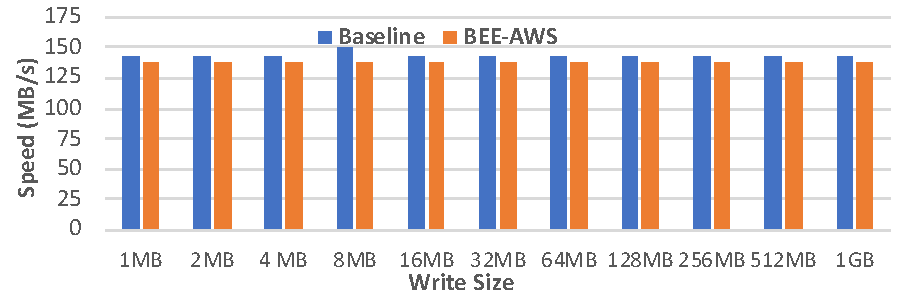
\includegraphics[width=\textwidth]{figures/write-bee-aws.pdf}
        \caption{Write Performance}
    \end{subfigure}
    
    %\vspace*{-0.5em}
    \caption{Comparison of storage I/O (\texttt{BEE-AWS}).}
    \label{io-aws}
   % \vspace*{-2em}
\end{figure}

\begin{figure}[t]
    \centering
    \begin{subfigure}[t]{0.5\textwidth}
        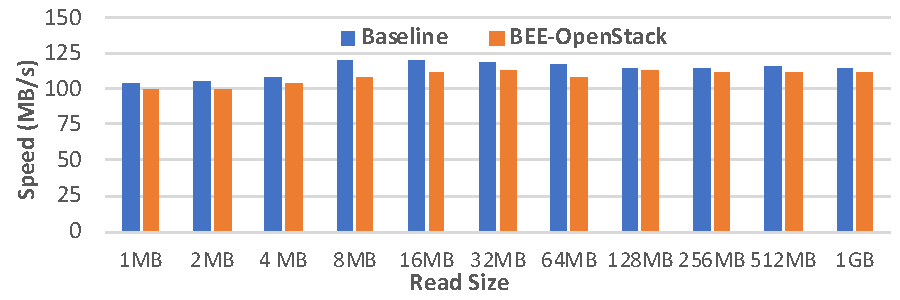
\includegraphics[width=\textwidth]{figures/read-bee-os.pdf}
        \caption{Read Performance}
    \end{subfigure}
    \begin{subfigure}[t]{0.5\textwidth}
        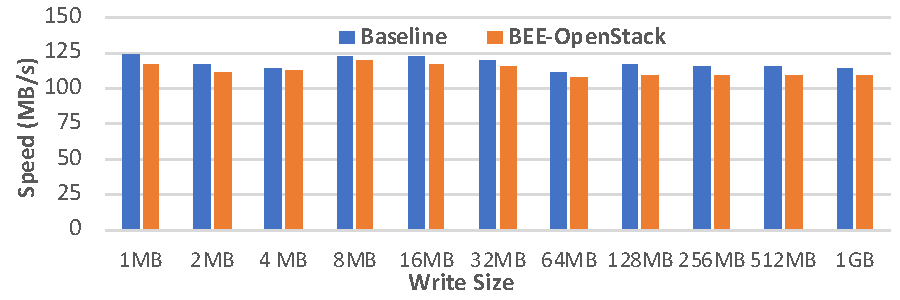
\includegraphics[width=\textwidth]{figures/write-bee-os.pdf}
        \caption{Write Performance}
    \end{subfigure}
    %\vspace*{-0.5em}
    \caption{Comparison of storage I/O (\texttt{BEE-OpenStack}).}
    \label{io-os}
   % \vspace*{-2em}
\end{figure}


\end{comment}





\section{Vector Particle-In-Cell Case Study}
  \label{sec:case_study}
 % \subsection{Vector Particle-In-Cell (VPIC)}
  In this section, we showcase an example running real HPC applications in \texttt{BEE-VM} on a production HPC machine. We test Vector Particle-In-Cell (VPIC) plasma physics code \cite{bowers20080, bowers2008ultrahigh, bowers2009advances} on \texttt{BEE-VM}. VPIC is a general purpose particle-in-cell plasma simulation code for modeling kinetic plasmas in multiple spatial dimensions. VPIC is memory bound application that runs on multiple nodes using MPI and pthreads. It has been optimized for modern computing architectures by using short-vector, single-instruction-multiple-data (SIMD) instructions and cache optimization. Before the simulation begins, VPIC needs to load input deck and user configuration files. When computation is finished, VPIC writes the output. With flexible checkpoint-restart semantics,  VPIC allows checkpoint files to be read as input for subsequent simulations. Moreover, VPIC has a native I/O format that interfaces with the high-performance visualization software Ensight and Paraview. 

We evaluate the performance of VPIC on our \texttt{BEE} framework on an HPC system and a cloud computing system compared with its performance on bare metal HPC systems. For the HPC system, we use our testbed cluster system Darwin. It has a `Galton` node partition (each `Galton node` has two NICs), which have KVM enabled. Each node has two 8-core Intel Ivy Bridge E5-2650 v2 CPUs with 251GB RAM. For the cloud  system, we use AWS EC2. On AWS, we choose to use \texttt{c3.4xlarge} instance type for each node on the cluster we deployed on AWS. Each node is equipped with Intel Xeon E5-2680 v2 CPUs with 16 vCPU cores and 30GB RAM. On Chameleon Cloud, we choose to deploy \texttt{BEE} on top of the SR-IOV enabled cluster. Each node in the cluster has two Intel Xeon E5-2670 v3 CPUs, 125GB RAM, and one Mellanox Infiniband card.


\begin{figure}[h]
    \centering
    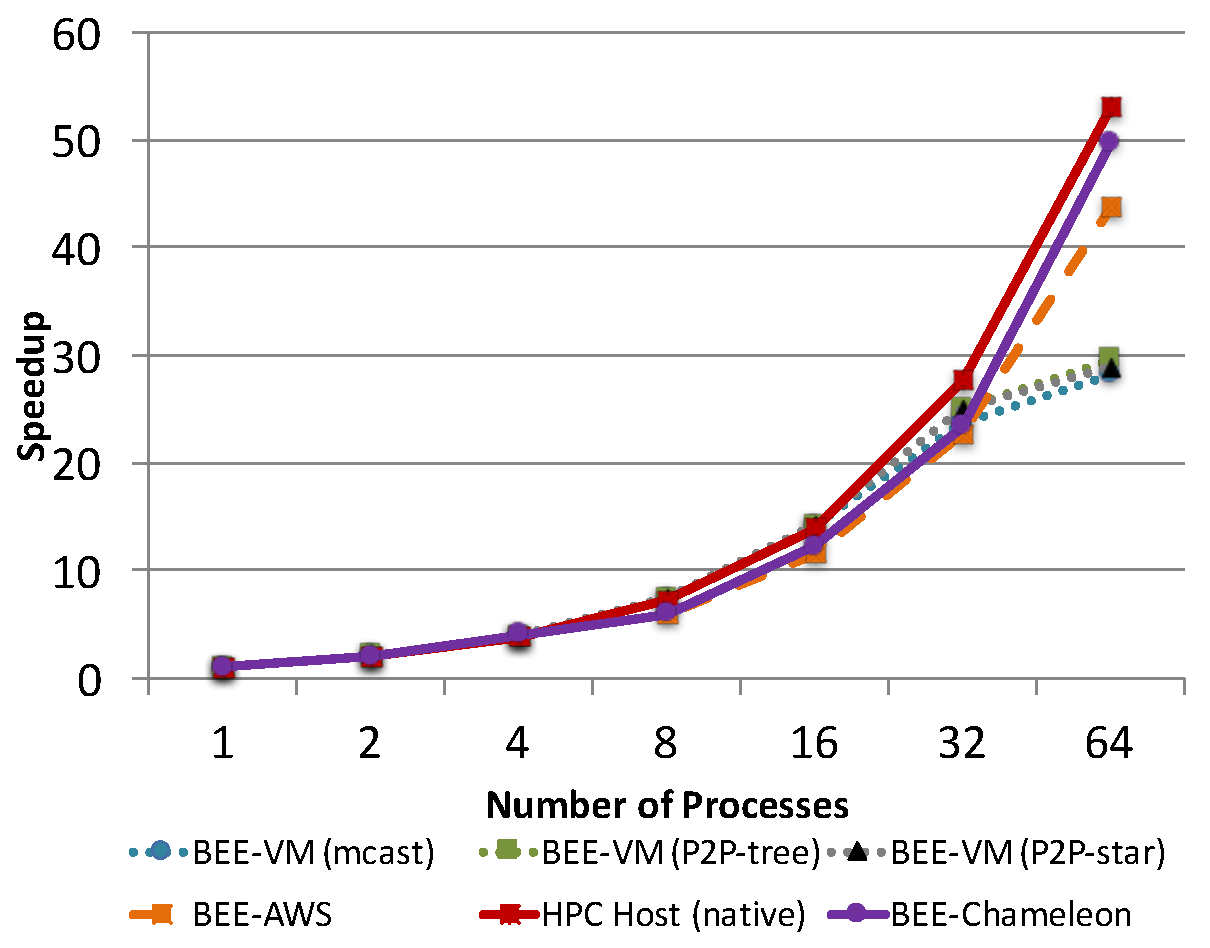
\includegraphics[width=0.5\textwidth]{figures/vpic-test.pdf}
    \caption{VPIC scale up test on \texttt{BEE-VM}, \texttt{BEE-AWS}, \texttt{BEE-Chameleon}, and HPC host. Results show that \texttt{BEE-AWS} and \texttt{BEE-Chameleon} scales similar to HPC native. \texttt{BEE-VM} also scales well under 64 processes, but with lower speedup.}
    \label{vpic-test}
    %\vspace*{-2em}
\end{figure}

We tested VPIC on different environments using 1 to 64 processes. As shown in \textbf{Fig. \ref{vpic-test}}, \texttt{BEE-AWS} and \texttt{BEE-Chameleon} solution scales similarly to the native host.  Our \texttt{BEE-VM} solutions (BEE-mcast, BEE-P2P-tree, and BEE-P2P-star) also scale well from 1 to 64 processes. Among all three network configurations, the tree-shaped connection using P2P sockets works the best. Since in VPIC, one-to-one process communication is much more frequent than all-to-all broadcast, tree-shaped connection can greatly mitigate the hot spot problem under this kind of communication pattern, as discussed before. Depending on the communication pattern in different applications, they may work best with different network designs. Due to the overhead of virtualized network, communication intensive applications, such as VPIC, scale up slower on \texttt{BEE-VM} than on native HPC hosts beyond 64 processes. We will continue to optimize the network performance (e.g., vNIC configuration, connection styles, topology, etc.).

\begin{comment}
\section{BEE in Workflow}
%\jchen{explain how we can integrate workflow logic in to \texttt{BEE}}
By encapsulating the computation provided by HPC (through \texttt{BEE-VM}) or cloud computing systems into containers and separating computation (the container) from state (the data mounts) workflows can be easily composed. Containers are treated as modules that can be easily assembled to form a large workflow system as needed. This enables users to easily build their workflow logic into \texttt{BEE}. Once a user has set the workflow logic,  \texttt{BEE} can deploy and manage user application according to the logic. For example, as shown in \textbf{Figure \ref{workflow}}, when a user wants to a series of pipelined simulations, the user needs to manually configure and start each simulation one by one and also needs to handle data transfer for the pipeline logic. If the pipeline consists of many simulations, it can be considerably difficult to manually deploy and debug, especially when different simulations are conducted on different hosts. However, by using \texttt{BEE}, the user only needs to indicate which simulations need to run and which one follow the other, then \texttt{BEE} can deploy simulation applications in orders and setup the pipeline data transfer. The containerized environment also allows the user to change certain parts of workflow logic at runtime as long as it does not interrupt normal execution.
 %For example, during the pipelined simulation, some soft error or bug occurs and causes incorrect final output data. 
 In-situ analysis as a new approach to diagnose the problem by checking out the intermediate resluts between successive simulation can also be containerized and plug into the workflow. Instead of running the filters and moving data to compete for the computation cycles and I/O bandwidth, In-situ visualization tools can be deployed seperately from the computation codes.  \texttt{BEE-VM} `s I/O design faciliates the in-situ analysis by allowing applying different filters even at the same time to process the data for visualization.
 
Continuous Integration(CI) \cite{fowler2006continuous} has been widely used in many HPC application development process. It is used for unit testing, fixing compatibility issues during integration, etc. Many development projects choose to use standard Docker image as output application format. Since \texttt{BEE} takes standard Docker images as input, it can be seamlessly integrated into CI development.
\begin{figure*}[h]
    \centering
    \caption{BEE with Workflow Integration}
    \label{workflow}
    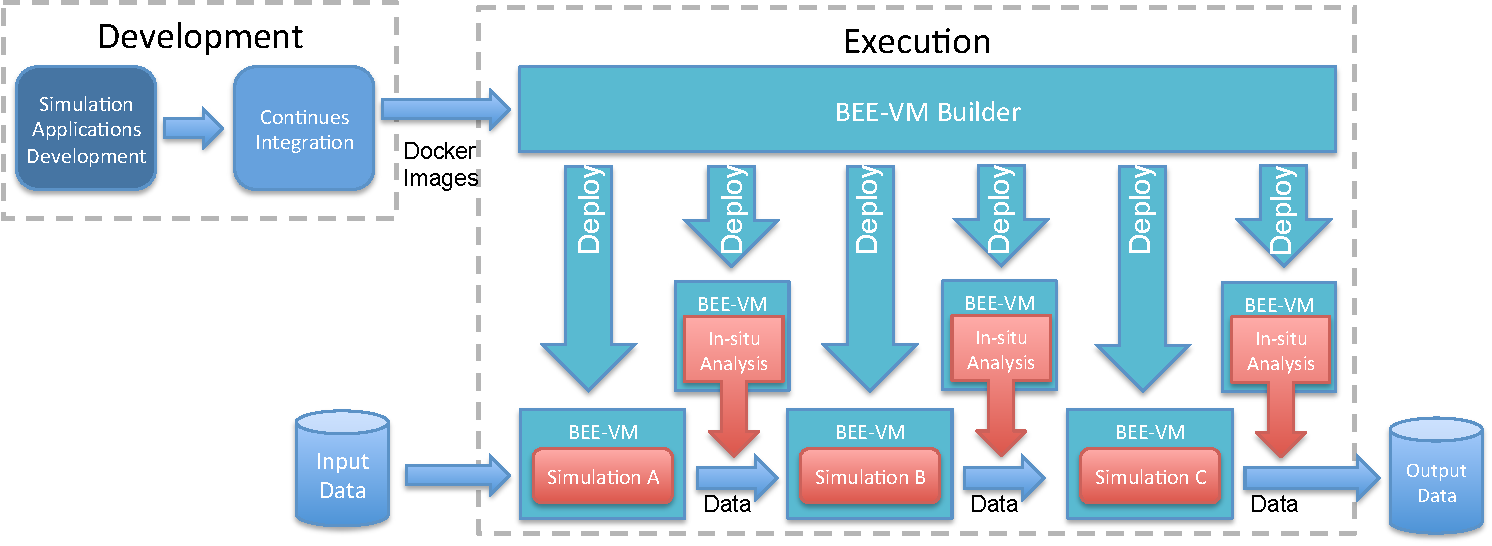
\includegraphics[width=0.75\textwidth]{figures/workflow.pdf}
    \vspace*{-2em}
\end{figure*}

\end{comment}
\section{Related Work}
\label{sec:RelatedWork}
Containers provide an opportunity to leverage cloud and industry software and practices within the HPC environment. However, various restrictions on current HPC system software and security policies limit the use of industry standard container technologies to execute applications on HPC platforms. Multiple efforts are underway within the DoE laboratories to provide solutions that ameliorate these issues (e.g., Shifter\cite{jacobsen2015contain}, Charliecloud\cite{kurtzer_2016_60736}, Singularity\cite{priedhorsky2016charliecloud}, and \texttt{BEE-VM}) and enable containers to execute securely on HPC platforms. 

Shifter is an execution environment that also aims to provide containerized environments for HPC systems. Since deploying the standard Docker daemon on HPC systems imposes security and compatibility issues, they build a Docker-like container environment, which provides portability, isolation, and reproducibility like Docker. Shifter runs customized Shifter images. Docker users need to first import their Docker images and convert them into Shifter images before running. Shifter containers can access the host file system via volume mapping; however, there is no explicit application data management. Also, sharing files between containers requires the file sharing abilities between host machines. Shifter can only be installed on customized Cray machines with root privileges, whereas \texttt{BEE} can run standard Docker images unmodified. Using \texttt{BEE} is easier for developers to ensure consistent environments across their local development and test machines along with production systems. Using standard Docker brings more convenience to develop and distribute Docker images in Docker communities. \texttt{BEE} has explicit application data management that can facilitate easy transfer across host machines for live migration or work flow integration. Also, \texttt{BEE-VM} has several modes for data file sharing between processes that can be configured by the user depending on whether file sharing is enabled on the hosts. If not, \texttt{BEE-VM} can build its own file sharing mechanism, which brings more flexibility. Finally, \texttt{BEE-VM} can be deployed on any HPC system and even cloud systems without root privileges. 

Singularity is another containerized execution environment for HPC systems. Similar to Shifter, it also build a Docker-like container execution environment to run customized Singularity images. Standard Docker images are supported but they also need to be converted to Singularity format before running. It is also required to have root privileges in order to install Singularity on HPC systems. Unlike Shifter, Singularity can be deployed on any HPC system. It does not seek to manage application data. Data sharing between containers also depends on the host filesystems. With multiple configuration solutions, \texttt{BEE} has more flexibility for deployment on HPC systems. Besides providing a containerized execution environment, \texttt{BEE} brings better usability by combining data management, workflow integration, live migration, and cloud computing together to provide a more convenient tool for HPC users and developers.

Charliecloud is a container solution that brings Docker-composed environments into HPC systems. It brings many of the benefits of standard Docker container; the main benefit  being that users or developers can have consistent building and execution environment from their local development and test machines to large scale production cluster machines. However, it is challenging to install Charliecloud on current HPC systems. Installing Charliecloud environment requires that the target HPC system has a Linux kernel version of at least 3.18.  This limitation constrains the current production HPC system ability to support Charliecloud. Moreover, it is only designed as the execution environment, many other aspects of HPC workflow have not been integrated.

While this paper details a specific \texttt{BEE} backend implementation, the \texttt{BEE-VM} and
\texttt{BEE-AWS}, there is nothing that precludes the addition of \texttt{BEE-Shifter}, \texttt{BEE-Singularity}, or \texttt{BEE-Charliecloud} backends for specific platforms.

Amazon EC2 Container Service (ECS) \cite{awscontainer} is a Docker container service provided by Amazon on AWS. Since ECS deploys on top of EC2, and EC2 has a layer on VMs, ECS actually deploys the Docker container layer on top of the VM layer, providing a similar host-VM-Docker structure as \texttt{BEE-VM}. Regardless of the underlying hardware configuration, ECS provides a consistent building and execution environment by using standard \texttt{BEE}. Docker users can easily run their application on ECS without modification. This allows us to deploy the similar structure on both cloud and HPC environment in \texttt{BEE}. 
  


%\section{Future Work}
%    \label{sec:discussion}
%In the next stage of this work, we will focus on several parts. First, we will continue to optimize the performance of \texttt{BEE-VM} in terms of I/O, network and computational performance. Second, we will continue to improve our \texttt{BEE} framework. We will add more flexible and adaptive scheduling strategies and more sophisticated resource management systems. Third, our current work can only utilize general CPUs, we will extend our \texttt{BEE} framework to utilize accelerators such as GPUs and Intel Xeon Phi, since these are commonly used in HPC application. Finally, we will Integrate system level checkpoint/restoration capability into \texttt{BEE}. It can greatly benefit applications that do not provide native application level checkpoint/restoration capabilities.

\section{Conclusions}
In this work, we first address the importance of the new in-situ analysis workflows. Next, we proposed \texttt{BeeFlow}, an in-situ analysis enabled workflow management system across HPC and cloud platforms with Docker support. We showed how we designed and optimized \texttt{BeeFlow} in the five-layer functionality architecture and evaluated the usability and performance. Moreover, we showcased three commonly used scientific workflows on \texttt{BeeFlow}. Finally, we compared \texttt{BeeFlow} with current existing workflow systems in multiple aspects and show that \texttt{BeeFlow} can be easily adopted to launch modern in-situ workflows in our case studies. Comparisons also showed that \texttt{BeeFlow} brings much better usage complexity and user time cost compared with manual approach and similar results compared to existing commonly used workflow tools. 



%\patg{This just tells what you did you should also state what the comparisons todl you in a concise manner, why use BeeFlow?}


\section{Acknowledgement}
This work was funded by the the US Government contract DE-AC52-06NA25396 for Los Alamos National Laboratory, operated by Los Alamos National Security,
LLC, for the US Department of Energy. This work was also supported by NSF Award No. 1513201. Results presented in this paper were obtained using the Chameleon Cloud sponsored by the National Science Foundation. The publication has been assigned the LANL identifier LA-UR-18-27912.

%\let\oldbibliography\thebibliography
%\renewcommand{\thebibliography}[1]{\oldbibliography{#1}
%\setlength{\itemsep}{0pt}} %Reducing spacing in the bibliography.

\bibliographystyle{IEEEtran}
%\bibliographystyle{ACM-Reference-Format}
\bibliography{refer} 

\end{document}
